\chapter{Higgs boson fiducial cross sections in the $H \rightarrow \gamma\gamma$ channel}
\label{capitolo_5}
In this section the differential cross sections for Higgs boson decaying production into the two-photons channel are measured, using 139 fb$^{-1}$ of full Run2 proton-proton collisions recorded at a center-of-mass energy of $\sqrt{s} = 13$ TeV by the ATLAS experiment at the Large Hadron Collider during the period 2015-2018. Analyses with smaller dataset at center-of-mass energy of $\sqrt{s} = 13$ TeV for both ATLAS and CMS experiments are in \cite{Aaboud_measurements, collaboration2018MeasurementAI}. The differential cross section measurements are separately performed for a set of variables, considering several quantities of the di-photon system and the jets kinematics and of the jets multiplicity produced with the Higgs boson\footnote{No separation has been done distinguishing the Higgs boson production modes. Actually the measured cross sections are inclusive in the production.}. 
The variables used in this work are presented down below:
\begin{itemize}
\item $p_T^{\gamma\gamma}$: The transverse momentum of the Higgs boson, measured with the di-photon system;
\item $|y_{\gamma\gamma}|$: The absolute rapidity of the Higgs boson, measured with the di-photon system;
\item $N_{\text{jets}}^{30}$: The multiplicity of jets associated with the Higgs boson production;
\item $p_T^{j1, 30}$: The transverse momentum of the highest-$p_T$ leading jet;
\item $m_{jj}^{30}$: The invariant mass of the two leading jets;
\item $\Delta \phi_{jj}$: The azimuthal angular difference of the two leading jets.
\end{itemize}
The flag '$30$' stands for the requirement for jets to have $p_T > 30 \text{GeV}$ to be selected for the analysis. The binning intervals for each quantity in the analysis is shown in Table \ref{binning_table}.
\\
The $p_T^{\gamma\gamma}$ distribution is sensitive to the bottom and charm quark Yukawa couplings of Higgs boson \cite{Bishara_2017}, while in the high-transverse-momentum region has a sensitivity to new heavy particles coupling to the Higgs boson. The $|y_{\gamma\gamma}|$ distribution is particularly responsive to the modeling of the production mechanism and to the parton distribution functions (PDF) of the colliding protons. The $p_T^{j1}$ distribution is sensitive  to the relative contributions of the different Higgs production mechanism, while the $m_{jj}$ distribution has sensitivity to the Vector Boson Fusion (VBF) production mechanism. Finally, the angular variable $\Delta \phi_{jj}$ is sensitive to the spin and CP quantum numbers of the Higgs boson.
\\\\
The measurements are performed in a fiducial region, definited by two isolated photons with transverse momentum greater than 35\% and 25\% of the total diphoton invariant mass for the leading and sub-leading photons respectively, each in a pseudorapidity region of $|\eta| < 1.37$ or $1.52 < |\eta| < 2.37$. Considering moreover the jets-related events, the constraints on jets require to have a transverse momentum $p_T > 30$ GeV and rapidity $|y| < 4.4$. The photon isolation is required to ensure to avoid the jets's fake rate wrongly classified as photons.
\\
The $H \rightarrow \gamma\gamma$ signal yield in each bin of the variable of interest has been extracted from fits to the di-photon invariant mass spectrum, assuming the Higgs boson mass to be $125.09 \pm 0.24$ GeV \cite{Aad_2015}, and the measured cross sections are tuned applying corrections arising from experimental effects and considering the integrated luminosity of the dataset.
\begin{table}[h]
\centering
\small
\caption{Binning intervals for each observable studied in the analysis.}
\label{binning_table}
\begin{tabular}{l | cccccc}
Bin & $p_T^{\gamma\gamma}$ [GeV] & $|y|_{\gamma\gamma}$ & $p_T^{j1, 30}$ [GeV] & $\Delta\phi_{jj}$ & $N_j^{30}$ & $m_{jj}^{30}$ [GeV] \\
\hline
1 & $0-5$ & $0-0.15$ & $<2 \hspace{0.1cm}\text{jets}$ & $-3.15--1.57$ & $= 0$ & $0-170$ \\
2 & $5-10$ & $0.15-0.30$ & $0-30$ & $-1.57-0$ & $= 1$ & $170-500$ \\
3 & $10-15$ & $0.30-0.45$ & $30-60$ & $0-1.57$ & $= 2$ & $500-1500$ \\
4 & $15-20$ & $0.45-0.60$ & $60-90$ & $1.57-3.15$ & $\geq3$ & $1500-\infty$ \\
5 & $20-25$ & $0.60-0.75$ & $90-120$ & - & - & - \\
6 & $25-30$ & $0.75-0.90$ & $120-350$ & - & - & - \\
7 & $30-35$ & $0.90-1.20$ & $\geq350$ & - & - & - \\
8 & $35-45$ & $1.20-1.60$ & - & - & - & - \\
9 & $45-60$ & $1.60-2.40$ & - & - & - & - \\
10 & $60-80$ & - & - &  - & - & - \\
11 & $80-100$ & - & - & - & - & - \\
12 & $100-120$ & - & - &  - & - & - \\
13 & $120-140$ & - & - & - & - & - \\
14 & $140-170$ & - & - & - & - & - \\
15 & $170-200$ & - & - & - & - & - \\
16 & $200-250$ & - & - & - & - & - \\
17 & $250-350$ & - & - & - & - & - \\
18 & $350-\infty$ & - & - & - & - & -
\end{tabular}
\end{table}

\section{Dataset and events simulation}
\label{mc_sim}
The analysis is based on $\sqrt{13}$ TeV proton-proton collisions, recorded from 2015 to 2018 with a proton bunch spacing of 25 ns. Because of the different luminosities reached during the data taking, the average number of interactions per bunch crossing varies from 24 in 2015-2016 to 37 in 2017-2018 data, leading to an average number of interaction per bunch crossing $\mu=34$.Prompt events are selected by using a diphoton trigger with $p_T$ threshold of 35 GeV and 25 GeV for the leading and sub-leading photon candidates respectively. Loose photon identification requirements are applied by the diphoton trigger in the 2015-2016 dataset and upgraded to tight requirements to deal with the higher instantaneous luminosity in the 2017 dataset, bringing the total identification efficiency of the diphoton trigger greater than 98\% for $H \rightarrow \gamma\gamma$ events passing the selections described below.
\\
After the data quality requirements achievement to ensure good working condition for all detector's sub-systems, the final integrated luminosity for the merged dataset settles down to $(139.0 \pm 2.4)$ fb$^{-1}$ \cite{ATLAS-CONF-2019-021}.
\\
The study of the backgroung and signal processes modelling is done using samples produced with MonteCarlo simulations. The background simulation is used to select the best functional form to fit the data and to estimate the systematic uncertainties related to the signal extraction due to the background mismodelling, such as the spurious signal (Section \ref{spur_sign_sec}). The $H \rightarrow \gamma\gamma$ signal simulation, on the other hand, is needed to determine the mass shape and the efficiencies for both \emph{c-factors} method (Section \ref{c_factors_sec}) and \emph{matrix} method (Section \ref{matrix_sec}).
\begin{table}[h]
\caption{MonteCarlo signal samples used in the analysis. The order listed for the QCD and EW calculations refers to the order to which the samples are normalized.}
\label{signal_samples}
\begin{center}
\begin{tabular}{ c | c | c | c}
  Process & Generator & Cross-section normalization & $\sigma \times \text{BR}$[fb] \\
  \hline			
  ggF & P{\scriptsize OWHEG} NNLOPS & N$^3$LO(QCD)+NLO(EW) & 110 \\
  VBF & P{\scriptsize OWHEG}-B{\scriptsize OX} & approx. NNLO(QCD)+NLO(EW) & 8.58 \\
  $W^+H$ & P{\scriptsize OWHEG}-B{\scriptsize OX} & NNLO(QCD)+NLO(EW) & 1.90 \\
  $W^-H$ & P{\scriptsize OWHEG}-B{\scriptsize OX} & NNLO(QCD)+NLO(EW) & 1.21 \\
  $q\bar{q} \rightarrow ZH$ & P{\scriptsize OWHEG}-B{\scriptsize OX} & NNLO(QCD)+NLO(EW) & 1.73 \\
  $gg \rightarrow ZH$ & P{\scriptsize OWHEG}-B{\scriptsize OX} & NLO(QCD)+NLO(EW) & 0.28 \\
  $t\bar{t}H$ & P{\scriptsize OWHEG}-B{\scriptsize OX} & NLO(QCD)+NLO(EW) & 1.15 \\
  $b\bar{b}H$ & P{\scriptsize OWHEG}-B{\scriptsize OX} & NLO(QCD)+NLO(EW) & 1.10
\end{tabular}
\end{center}
\end{table}
\\The signal samples used in the analysis are summarized in Table \ref{signal_samples}. The Higgs boson's mass is set in the simulations at $m_H = 125$ GeV with a width of $\Gamma_H = 4.07$ MeV and the $H \rightarrow \gamma\gamma$ branching ratio of $0.227 \%$ for a mass of the Higgs boson of $125.09$ GeV. All the main Higgs production modes are simulated separately.
\\\\
The ggF sample is generated with NNLOPS \cite{Hamilton_2013}, reaching an accordance in the $p_T$ and rapidity distribution for the Higgs boson compatible with that of next-to-next-to-leading order (NNLO) in QCD and it is normalized to N$^3$LO calculation (QCD) with additional NLO electroweak (EW) corrections \cite{Actis_2008ug, Anastasiou2018MixedQC, Bonetti_2018}. The PDF4LHC15 NNLO PDF \cite{Butterworth_2015oua} set and the AZNLO \cite{Aad_2014} tune of P{\scriptsize YTHIA}8 \cite{Sj_strand_2008} are used.
\\
The VBF sample is generated with P{\scriptsize OWHEG} \cite{Nason_2010} and combined with P{\scriptsize YTHIA}8 for parton showers' treatment and the non-perturbative effects. The sample is normalized to an approximate NNLO calculation in QCD with NLO electroweak corrections \cite{Ciccolini_2008, PhysRevLett_105_011801}. The PDF4LHC15 PDF set and the AZNLO tune of P{\scriptsize YTHIA}8 are used.
\\
The $WH$ or $ZH$ samples, typically known as $VH$, represent the Higgs boson production in association with a vector boson and are generated with P{\scriptsize OWHEG}-B{\scriptsize OX} \cite{Luisoni_2013}. This category contains several different samples separately produced: $W^+H$, $W^-H$, $q\bar{q} \rightarrow ZH$ and $gg \rightarrow ZH$ are generated with the next-to-leading order (NLO) matrix element matched to the parton shower , except for $gg \rightarrow ZH$, which is generated at leading order (LO). As well as for the VBF samples, also $VH$ samples are produced using PDF4LHC15 PDF set and AZNLO tune of P{\scriptsize YTHIA}8. All samples are normalized to NNLO in QCD with NLO electroweak corrections, except for the $gg \rightarrow ZH$ production mode, which is normalized only at NLO in QCD.
\\
The samples for two $t$-quarks associated Higgs boson productions ($t\bar{t}H$) is generated using P{\scriptsize OWHEG+}P{\scriptsize YTHIA}8 \cite{Hartanto2015HiggsBP}. This sample uses the PDF4LHC15 PDF set and the A14 generator tune. The normalization for the $t\bar{t}H$ sample reach the accuracy to NLO in QCD with NLO electroweak corrections \cite{Dawson_2003, Zhang_2014}.
\\
The $b\bar{b}H$ sample is generated with P{\scriptsize OWHEG}-B{\scriptsize OX} \cite{Jager2016HiggsBP} and contains additional NLO electroweak corrections, to take in consideration the quark-mass effects' treatment. The PDF4 LHC15 PDF set and the A14 NNPDF23LO generator tune of P{\scriptsize OWHEG+}P{\scriptsize YTHIA}8 are used.
\\\\
The background events' sample from continuum $\gamma\gamma$ production, not considering interference effects related with the $H \rightarrow \gamma\gamma$ signal, is generated using  S{\scriptsize HERPA} $2.2.4$ \cite{Bothmann_2019} and matched to the S{\scriptsize HERPA} parton shower according to ME+PS@NLO prescription \cite{H_che_2013, Catani2001QCDME}. The background sample exploit the NNPDF3.0 NNLO PDF set \cite{Ball_2015}.
\\\\
The pile-up effects in the same and in the neighbouring bunch crossing are shaped by the superposition of simulated inelastic $pp$ collision events generated with P{\scriptsize YTHIA}8 using NNPDF2.3LO as PDFs \cite{Ball_2013} set and the A3 tune \cite{ATL-PHYS-PUB-2016-017} over the original hard-scattering events.
\\\\
The samples generated in that way are processed with the G{\scriptsize EANT}4 framework \cite{AGOSTINELLI2003250}, simulating the passage of the particle within the ATLAS detector \cite{Aad_2010} and reproducing the response of the latter to the particle's crossing. The $\gamma\gamma$ background sample is simulated with a fast simulation where the calorimeter's response is simulated with a parametrisation \cite{ATLAS_1300517}.

\section{Fiducial definition of the $H \rightarrow \gamma\gamma$ cross section}
Due to the finite detector acceptance it is not possible to study the differential cross section in the full phase space. In order to not introduce extrapolation systematics, a fiducial region is considered at parton level.The two photons must fall in the detector acceptance, $|\eta| < 2.37$ and outside the region $1.37 < |\eta| < 1.52$. The fiducial selected photons are required to have an invariant mass in the range $105 \text{GeV} < m_{\gamma\gamma} < 160 \text{GeV}$ and to pass at the same time the $p_T^{\gamma}/m_{\gamma\gamma}$ kinematic threshold of $0.35$ and $0.25$ for the leading-$p_T$ and for the subleading-$p_T$ photons respectively.
\\
Particle-level isolation requirements are needed in the fiducial definition, in order to trace the isolation requirements on detector-reconstructed-level particles. Due to the particle-level isolation requirement, each photon must satisfy $\sum p_T^i / p_T^{\gamma} < 0.05$, where $\sum p_T^i$ is the transverse momentum sum of every particle with $p_T > 1$ GeV whitin a cone of radius $\Delta R = 0.2$ centered around the photon .
\\
Regarding the particle-level fiducial jets definition, they are constructed clustering all stable particles not considering muons and neutrinos, with the anti-$k_t$ algorithm whitin a cone of radius $\Delta R = 0.4$. As in the quantity definition for the analysis, particle-level jets are required to have $p_T > 30$ GeV and $|y| < 4.4$, as well as mantaining the separation requirement with photons ($\Delta R_{j,\gamma} > 0.4$), in order to not contain the selected isolated photons in the cone. In Figure \ref{fiducial} the action of the fiducial selection on every quantity under investigation in shown.
\begin{figure}[htb]
\centering
\subfloat{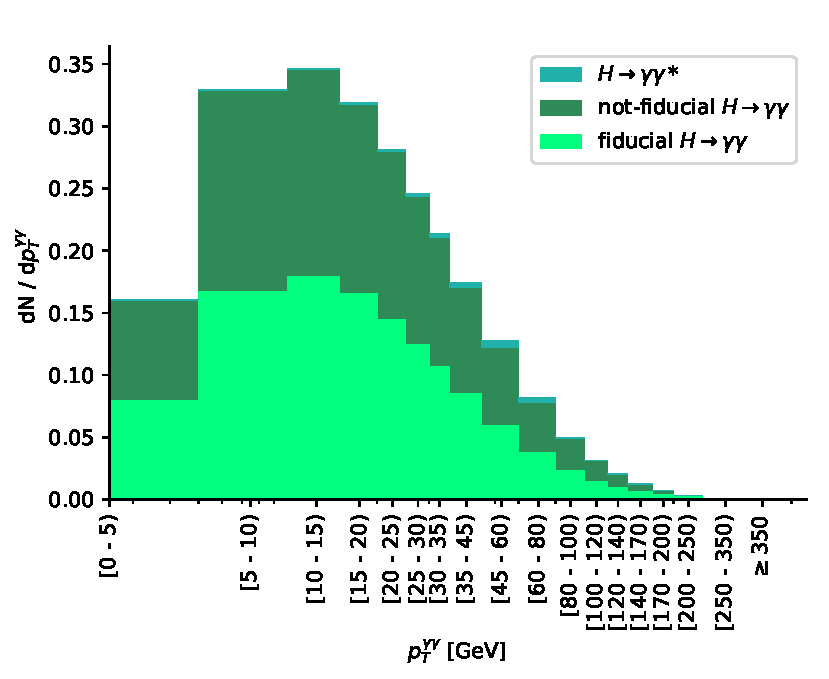
\includegraphics[scale=0.47]{stacked_pT_yy.pdf}}
\subfloat{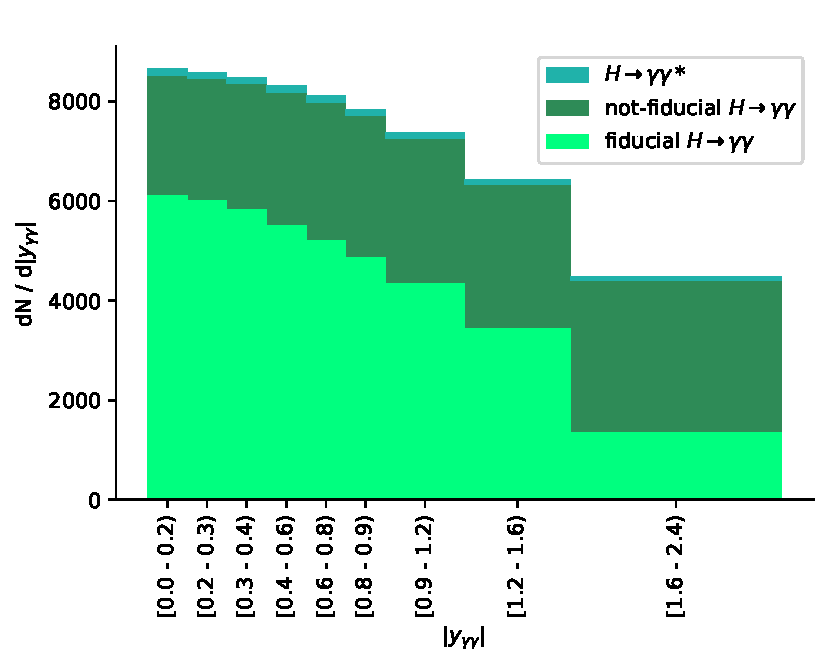
\includegraphics[scale=0.47]{stacked_yAbs_yy.pdf}} 
\end{figure}
\begin{figure}[ht]
\centering
\subfloat{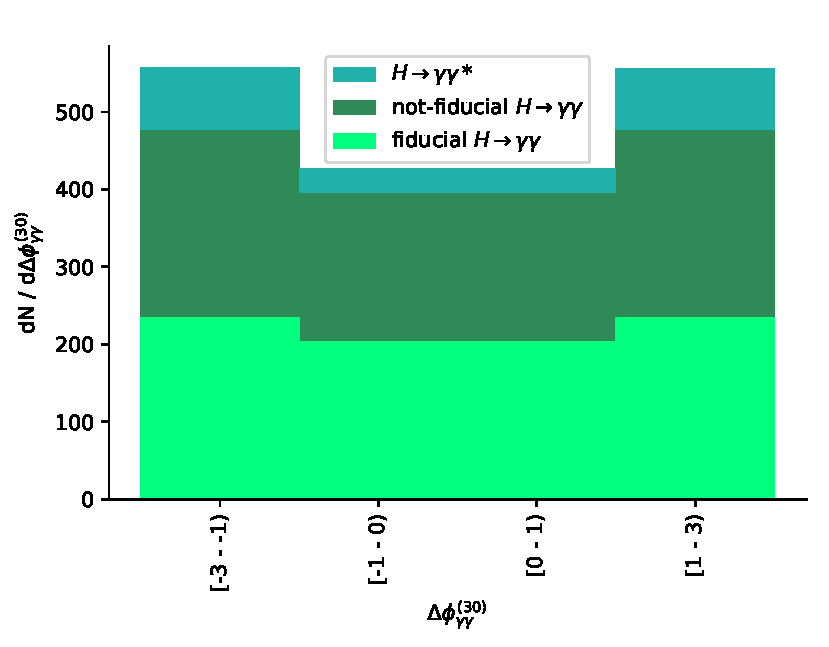
\includegraphics[scale=0.47]{stacked_Dphi_j_j_30_signed.pdf}}
\subfloat{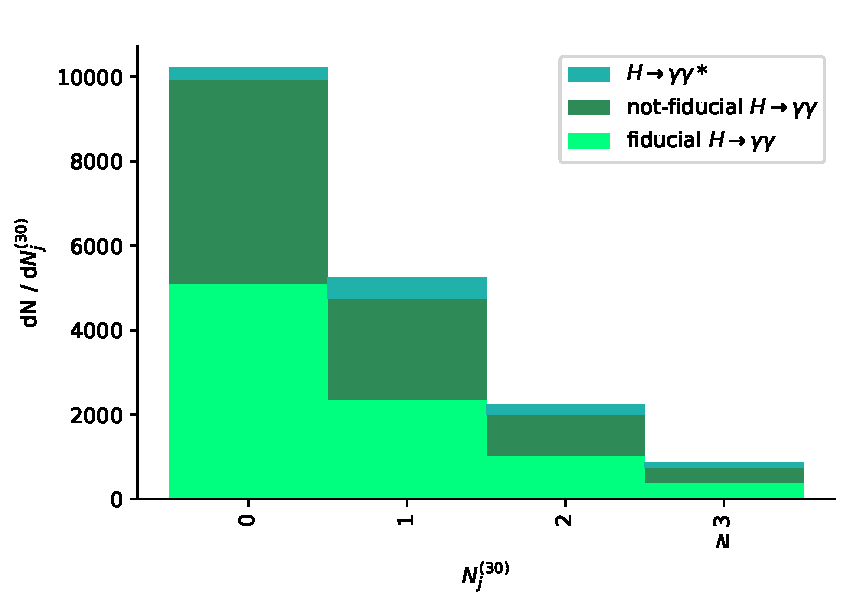
\includegraphics[scale=0.47]{stacked_N_j_30.pdf}} \\
\subfloat{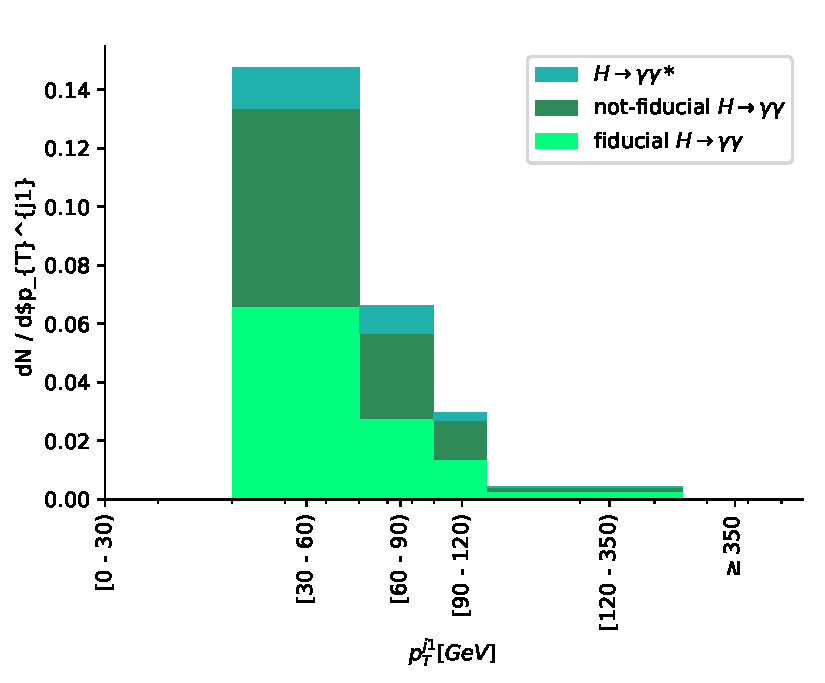
\includegraphics[scale=0.47]{stacked_pT_j1_30.pdf}}
\subfloat{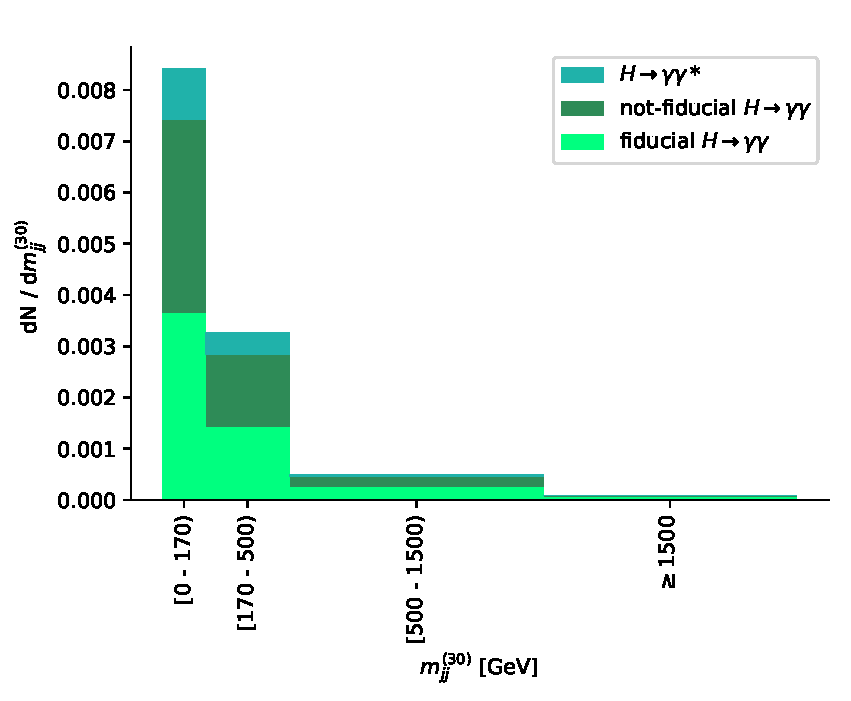
\includegraphics[scale=0.47]{stacked_m_jj_30.pdf}}
\caption{Distribution at true level for all the quantities under investigation. Also the not fiducial events and the Dalitz events are plotted. Notice how the fiducial cuts lower of about $50\%$ the number of events.}
\label{fiducial}
\end{figure}

\section{Event selection}
Collision events are reconstructed in the ATLAS detector by a series of algorithms previously discussed. Objects reconstructed as photons and jets are selected and collected in the analysis dataset.
\begin{itemize}
\item \emph{Photons}: reconstructed from Electromagentic Calorimeter's topo-clusters formed with topological clustering algorithm and classified as converted photons, if there isn't any corresponding track matching in the Inner Detector, or unconverted photons, if corresponding matching tracks are found in the Inner Detector. Reconstructed photons must satisfy $|\eta| < 2.37$ or $1.37 < |\eta| < 1.52$ to fall inside the Electromagnetic Calorimeter barrel or end-cap detecting regions. In order to suppress photons arising from hadrons jets, especially those deriving from $\pi^0 \rightarrow \gamma\gamma$ processes, shower-shape and isolation criteria are imposed, significately optimized for sub-ranges of photon's transverse momentum $p_T$. This $p_T$-dependence in the photons reconstruction and identification brings an efficiency greater than $82\%$ for a photon with $p_T > 25$ GeV. Further calorimeter- and track-based isolation requirements are applied, in order to suppress jets misidentified as photons: the isolation energy $E_T^{\text{iso}}$ is calculated as the transverse energy $E_T$ of the four-momentum sum of all charged particles which have $p_T > 1$ GeV within a cone of $\Delta R  = \sqrt{(\Delta\phi)^2 +(\Delta\eta)^2} < 0.2$ around the photon candidate, subtracting the contribution of the particle candidate and of the underlying and pile-up events. The diphoton system is rejected if the two selected photons do not satisfy $E_T^{\text{iso}} < 0.05 p_T$, while for the calorimeter-based isolation, the system must satisfy $E_T^{\text{iso}} < 0.065 p_T$. Both conditions are intended for each photon candidate of the diphoton system. After the diphoton system selection, the invariant mass of the diphoton system $m_{\gamma\gamma}$ is required to lie in the range $m_{\gamma\gamma} = [105, 160]$ GeV. The leading and sub-leading photons must satisfy the requirement $p_T/m_{\gamma\gamma} > 0.35$ and $p_T/m_{\gamma\gamma} > 0.25$ respectively; 
\\\\
Once the reconstruction process for all photons is performed, the two leading in $pT$ passing the loose identification criteria are selected and chosen as potential $H \rightarrow \gamma\gamma$ decay products. The vertex selection is obtained by using a dedicated neural network, properly trained by simulated ggF $H \rightarrow \gamma\gamma$ events to identify the primary hard interaction vertex in which the Higgs boson is produced. The vertex reconstruction algorithm has around $76\%$ chance of selecting the true Higgs vertex in terms of position resolution, corresponding to a distance uncertainty of $0.03$ mm from the real vertex \cite{ATL-PHYS-PUB-2015-026};

\item \emph{Jets}: reconstructed by clustering calorimeter topological clusters by using the anti-$k_T$ clustering algorithm with a radius parameter of $0.4$. Jets are rejected if they lie within $\Delta R = \sqrt{(\Delta\phi)^2 +(\Delta\eta)^2} < 0.4$ or $\Delta R = \sqrt{(\Delta\phi)^2 +(\Delta\eta)^2} < 0.2$ of a selected photon or selected electron respectively, to avoid the double-counting of the selected particles as jets. In addition, jets are required to have $p_T > 30$ GeV and $|y| < 4.4$, while jets with $|\eta| < 2.5$ and $p_T < 120$ GeV originating from pile-up collisions are suppressed using a jet vertex tagger multivariate discriminant \cite{ATLAS-CONF-2014-018, Aad_2016_pileup}.
\end{itemize}
\section{Signal and background modelling}
The analysis is based on fit of the $m_{\gamma\gamma}$ distribution in various categories, one for each bin to be measured. To do that, a model for the signal and for the background for each category is needed.
\\
Both signal and background modelling are discussed down below. The mass range considered in the analysis is $105 \text{GeV} < m_{\gamma\gamma} < 160 \text{GeV}$, in order to be wide enough to allow the determination of the background continuum from data, made by evaluating the sidebands to both sides of the resonant peak, but not too much to limit the uncertainties from the choice of the background parameterization function.

\subsection{Signal model}
The shape of the $m_{\gamma\gamma}$ for the signal is empirically modeled as a Double-Sided Crystal Ball (CB) function, a  commonly used in High Energy Physics PDF and consisting of a Gaussian core portion and power-law tails on both sided.

\begin{equation}
CB(m_{\gamma\gamma}) = N \times \begin{cases}
									e^{-t^2/2} \hspace{4cm} &\text{if} \hspace{0.2cm} -\alpha_{low} \leq t \leq \alpha_{high} \\
									e^{-\frac{1}{2}\alpha_{low}^2}\Bigl[\frac{1}{R_{low}}(R_{low} - \alpha_{low} - t)\Bigr]^{-n_{low}} \hspace{1cm} &\text{if} \hspace{0.2cm} t < -\alpha_{low} \\
									e^{-\frac{1}{2}\alpha_{high}^2}\Bigl[\frac{1}{R_{high}}(R_{high} - \alpha_{high} - t)\Bigr]^{-n_{high}} \hspace{0.7cm} &\text{if} \hspace{0.2cm} t < -\alpha_{high}
									\end{cases}							
\end{equation}
where
\begin{align}
&t = \frac{m_{\gamma\gamma} - \mu_{CB}}{\sigma_{CB}} \\
&R_{low} = \frac{\alpha_{low}}{n_{low}} \\
&R_{high} = \frac{\alpha_{high}}{n_{high}}
\end{align}
\begin{figure}[htb]
\centering
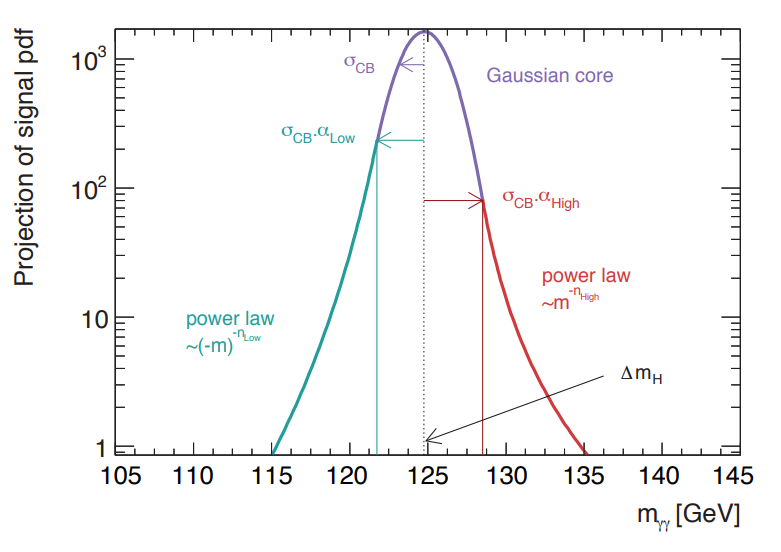
\includegraphics[scale=0.3]{DS_CB.png}
\caption{Example of a Double-Sided Crystal Ball function.}
\label{CB_example}
\end{figure}
and $N$ is the normalization factor, $\mu_{CB}$ is the mean of the Gaussian core distribution, $\sigma_{CB}$ is the width of the Gaussian core distribution, $\alpha_{low/high}$ are the position of the transition from the Gaussian core to the power-law tails on the low and high mass sides respectively and $n_{low/high}$ are the exponents of the low and high mass tails respectively. A detailed description of the procedure is described in \cite{Min_2309522}, while in Figure \ref{CB_example} an example of the Crystal Ball function is presented. 
\\
All the parameters of the Double-Sided Crystal Ball function are obtained by fitting a simulated $H \rightarrow \gamma\gamma$ decays dataset at $m_{\gamma\gamma} = 125$ GeV and then shifting the resonant peak by 90 MeV, in order to optimize the signal model for a Higgs boson with a mass of $125.09$ GeV. Being able to vary for the different bins, the value of each parameter is calculated for each bin of the variable in question. In Figure \ref{signal_param_example} the signal parameterisations for bins with the best and the worst resolution are shown. 
\begin{figure}[htb]
\subfloat[][]{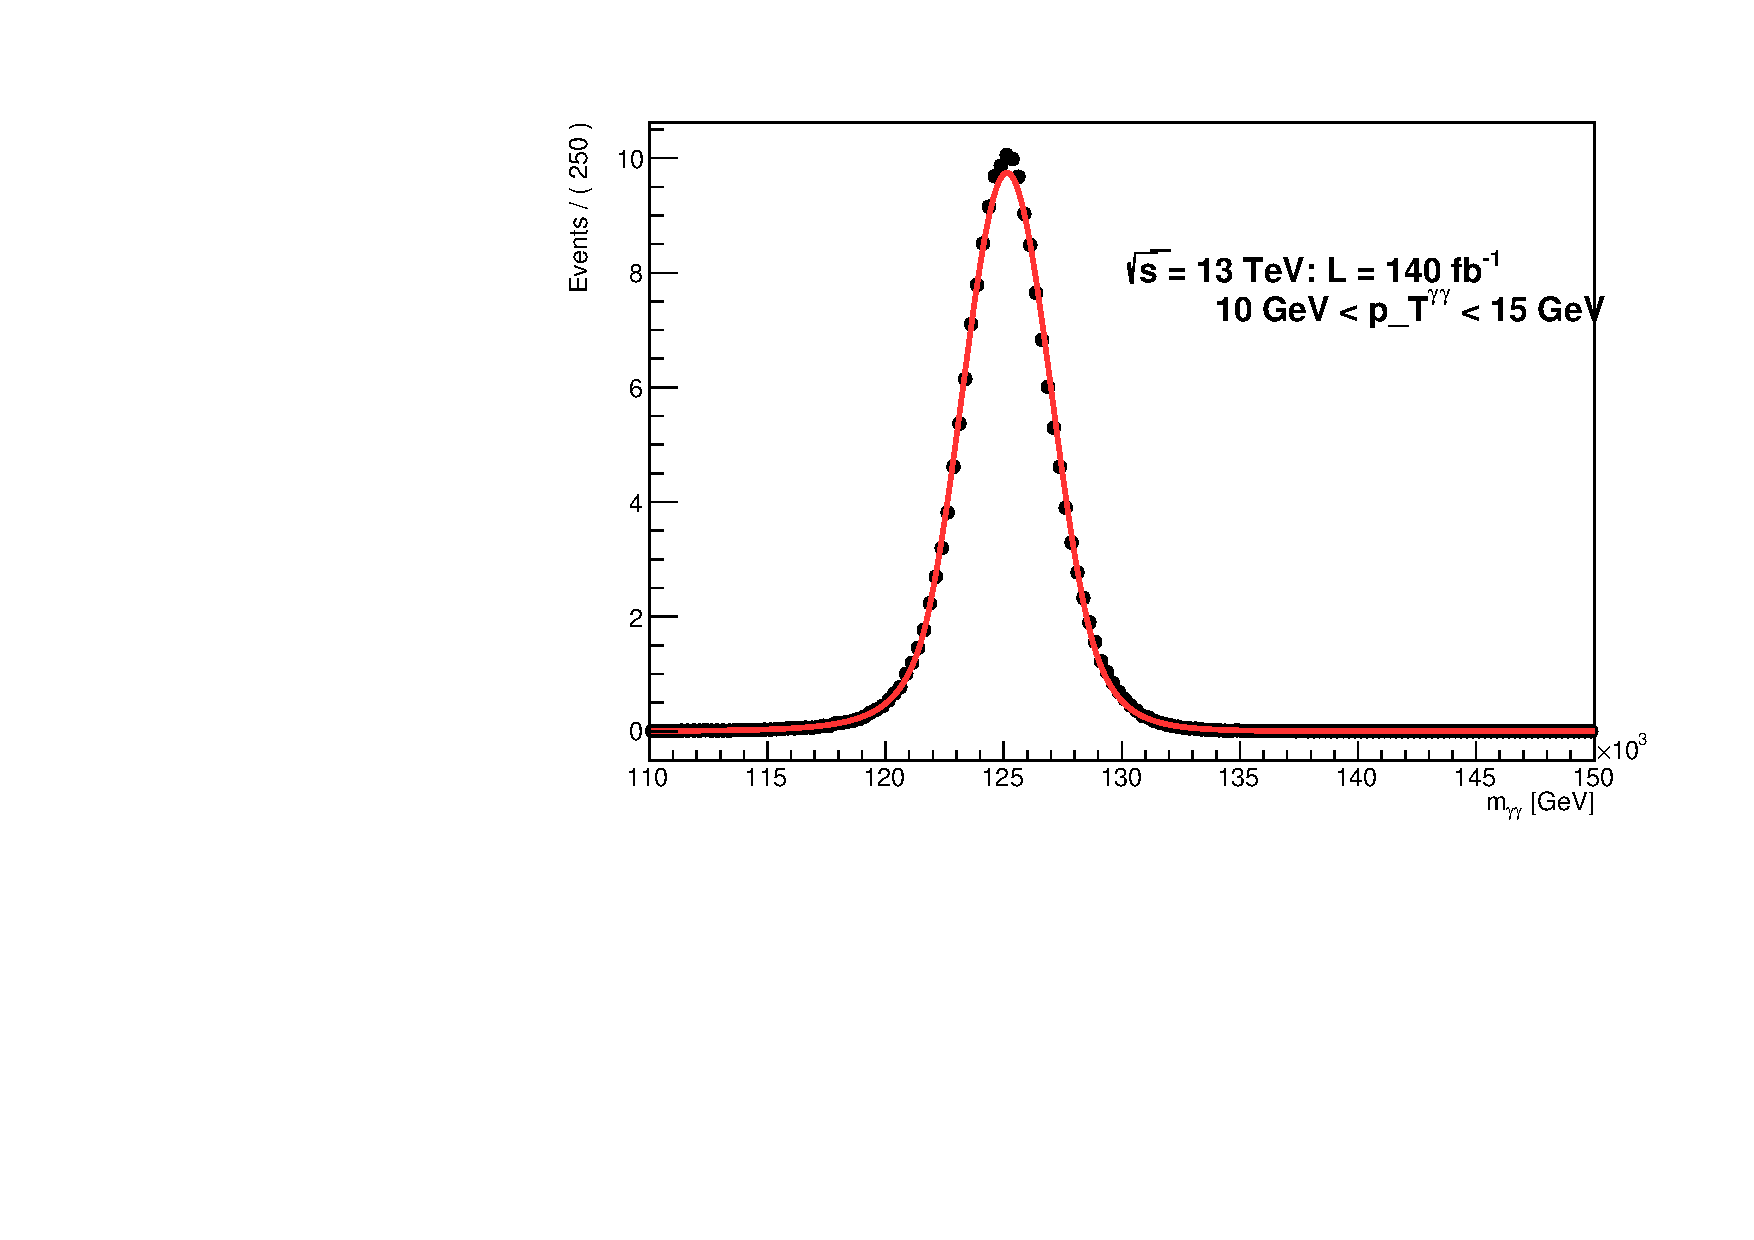
\includegraphics[scale=0.365]{signalParametrisation/fit_pT_yy_bin_3.pdf}}
\subfloat[][]{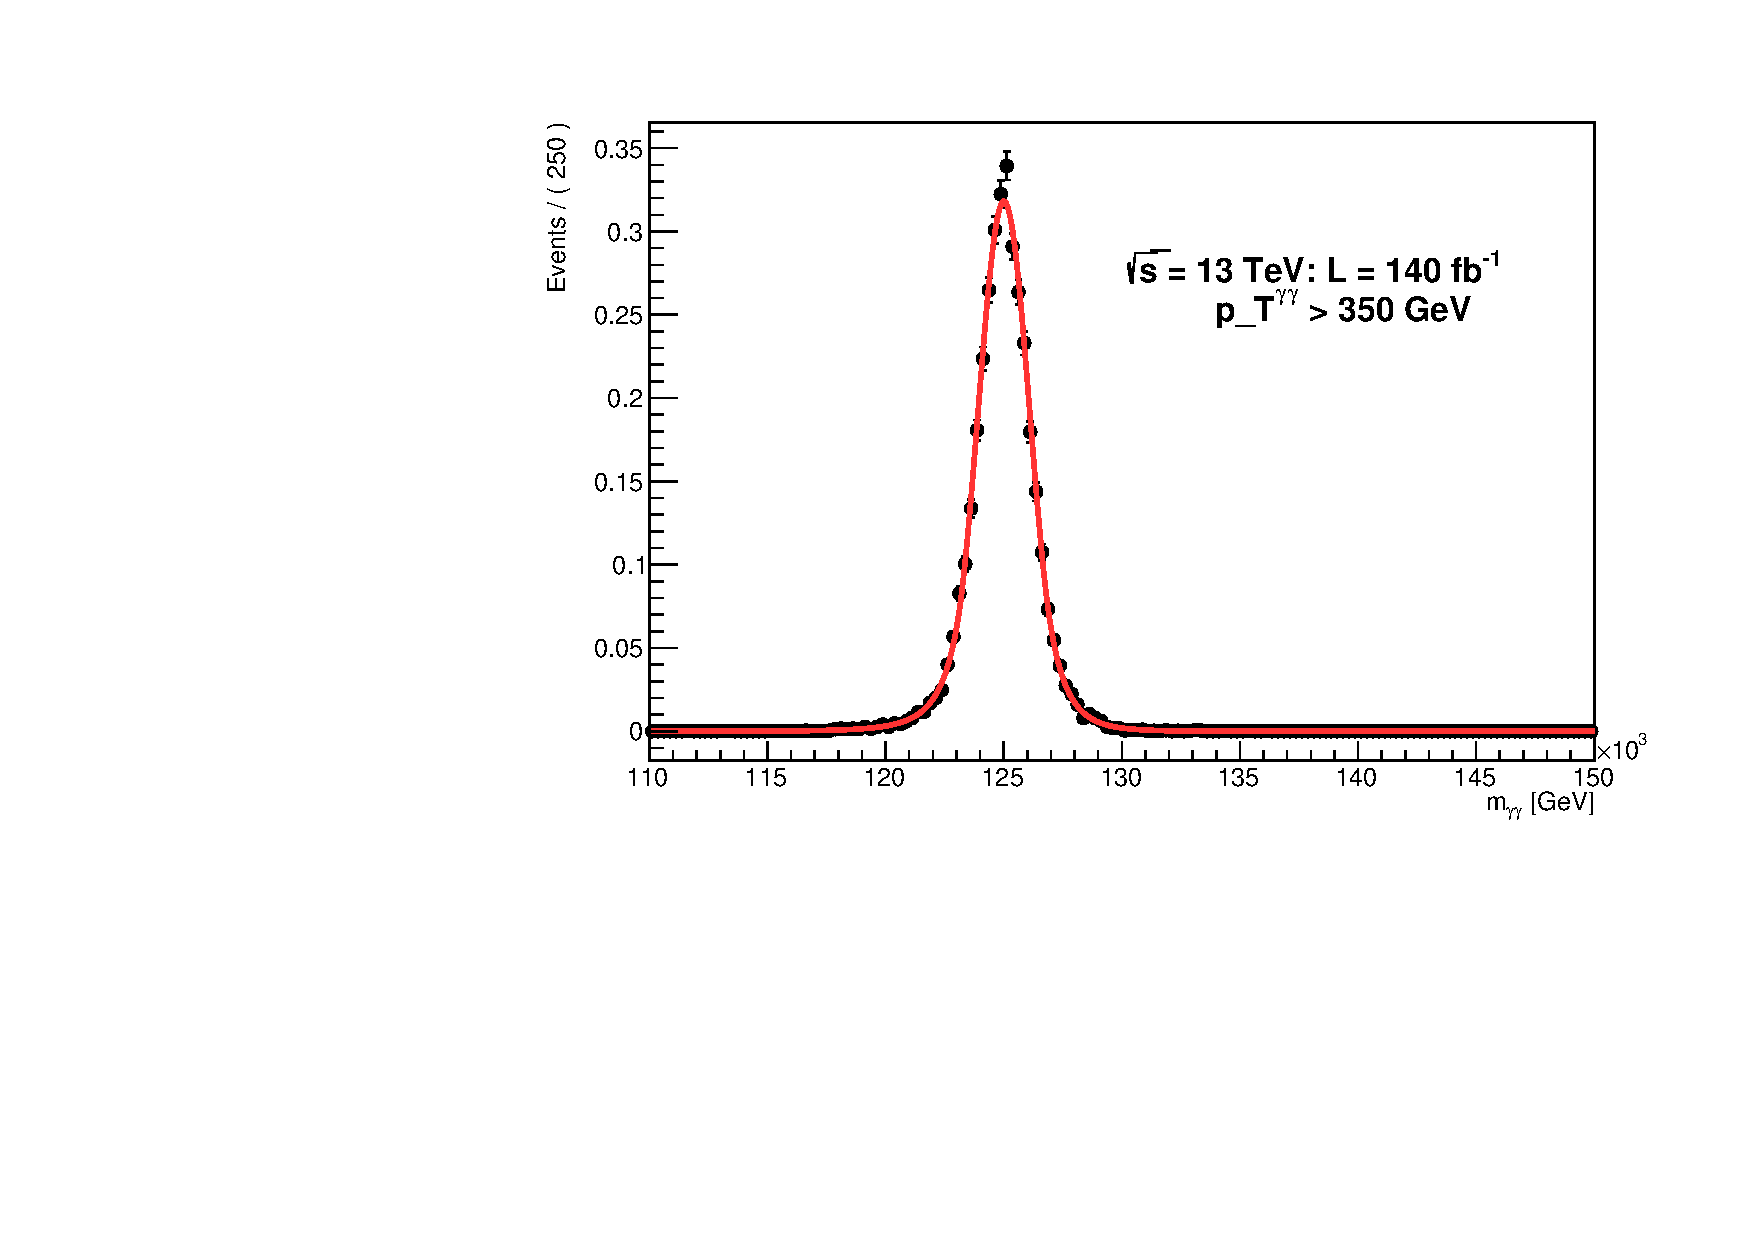
\includegraphics[scale=0.365]{signalParametrisation/fit_pT_yy_bin_18.pdf}}
\caption{a)Signal parameterisation for the fiducial dataset, normalized to $140$ fb$^{-1}$ and to the bin width for bin with the best resolution, b)Signal parameterisation for the fiducial dataset, normalized to $140$ fb$^{-1}$ and to the bin width for bin with the worst resolution. Plots for other observables and bins are shown in Appendix \ref{CB_plots_appendix}.}
\label{signal_param_example}
\end{figure}

\subsection{Background model}
The backgrounds continuum consists of three non resonant components, conforming to the different origin of the photon candidates: the $\gamma\gamma$ component includes selected isolated photons and it is simulated with the S{\scriptsize HERPA} event generator, while the $\gamma j$ and $jj$ components concern the cases where one or both photons candidates in the final state arise from hadronic jets misidentified as photons. The measurement of the background continuum fraction in data is obtained by using a double two-dimensional side-band fitting method for each cross section bin. Being the background distribution an empirically chosen functional form, the shape of the selected function may vary for each bin, incrementing the fit accuracy for each bin and consequently reducing the bias between the fitting function and the data through a spurious signal analysis, further discussed below. An example of background fitting function is shown in Figure \ref{bkg_example}. Several functional forms for the diphoton mass spectrum background are tested: exponentials of first (Exp) and second (ExpPoly$2$) degree polinomials and power law functions of first order (Pow).
\\
The exponential function is defined as 
\begin{equation}
B\Bigl(m_{\gamma\gamma}; \alpha_1^{\text{bkg}}\Bigr) = N\Bigl(\alpha_1^{\text{bkg}}\Bigr) \cdot \text{exp}\Bigl(-\frac{m_{\gamma\gamma}}{\alpha_1^{\text{bkg}}}\Bigr) \hspace{0.2cm} \text{,}
\end{equation}
while the second order exponential polynomial is defined as
\begin{equation}
B\Bigl(m_{\gamma\gamma}; \alpha_1^{\text{bkg}}, \alpha_2^{\text{bkg}}\Bigr) = N\Bigl(\alpha_1^{\text{bkg}}, \alpha_2^{\text{bkg}}\Bigr) \cdot \text{exp}\Bigl(-\frac{m_{\gamma\gamma}}{\alpha_1^{\text{bkg}}} - \frac{m_{\gamma\gamma}^2}{\alpha_2^{\text{bkg}}}\Bigr) \hspace{0.2cm} \text{,}
\end{equation}
where $\alpha_i^{\text{bkg}}$ are nuisance parameters and $N($\textbf{$\alpha^{\text{bkg}}$}$)$ is a normalization factor. In general, a higher-order exponential is preferred for bins with more events.
\\
Lastly, the first order power-law function is defined as
\begin{equation}
B\Bigl(m_{\gamma\gamma}; \alpha_1^{\text{bkg}}\Bigr) = N\Bigl(\alpha_1^{\text{bkg}}\Bigr) \cdot (m_{\gamma\gamma})^{\alpha^1}
\end{equation}
The choice of the background functional form is performed to minimize the bias due to potential mismodelling.
\begin{figure}[hbt]
\centering
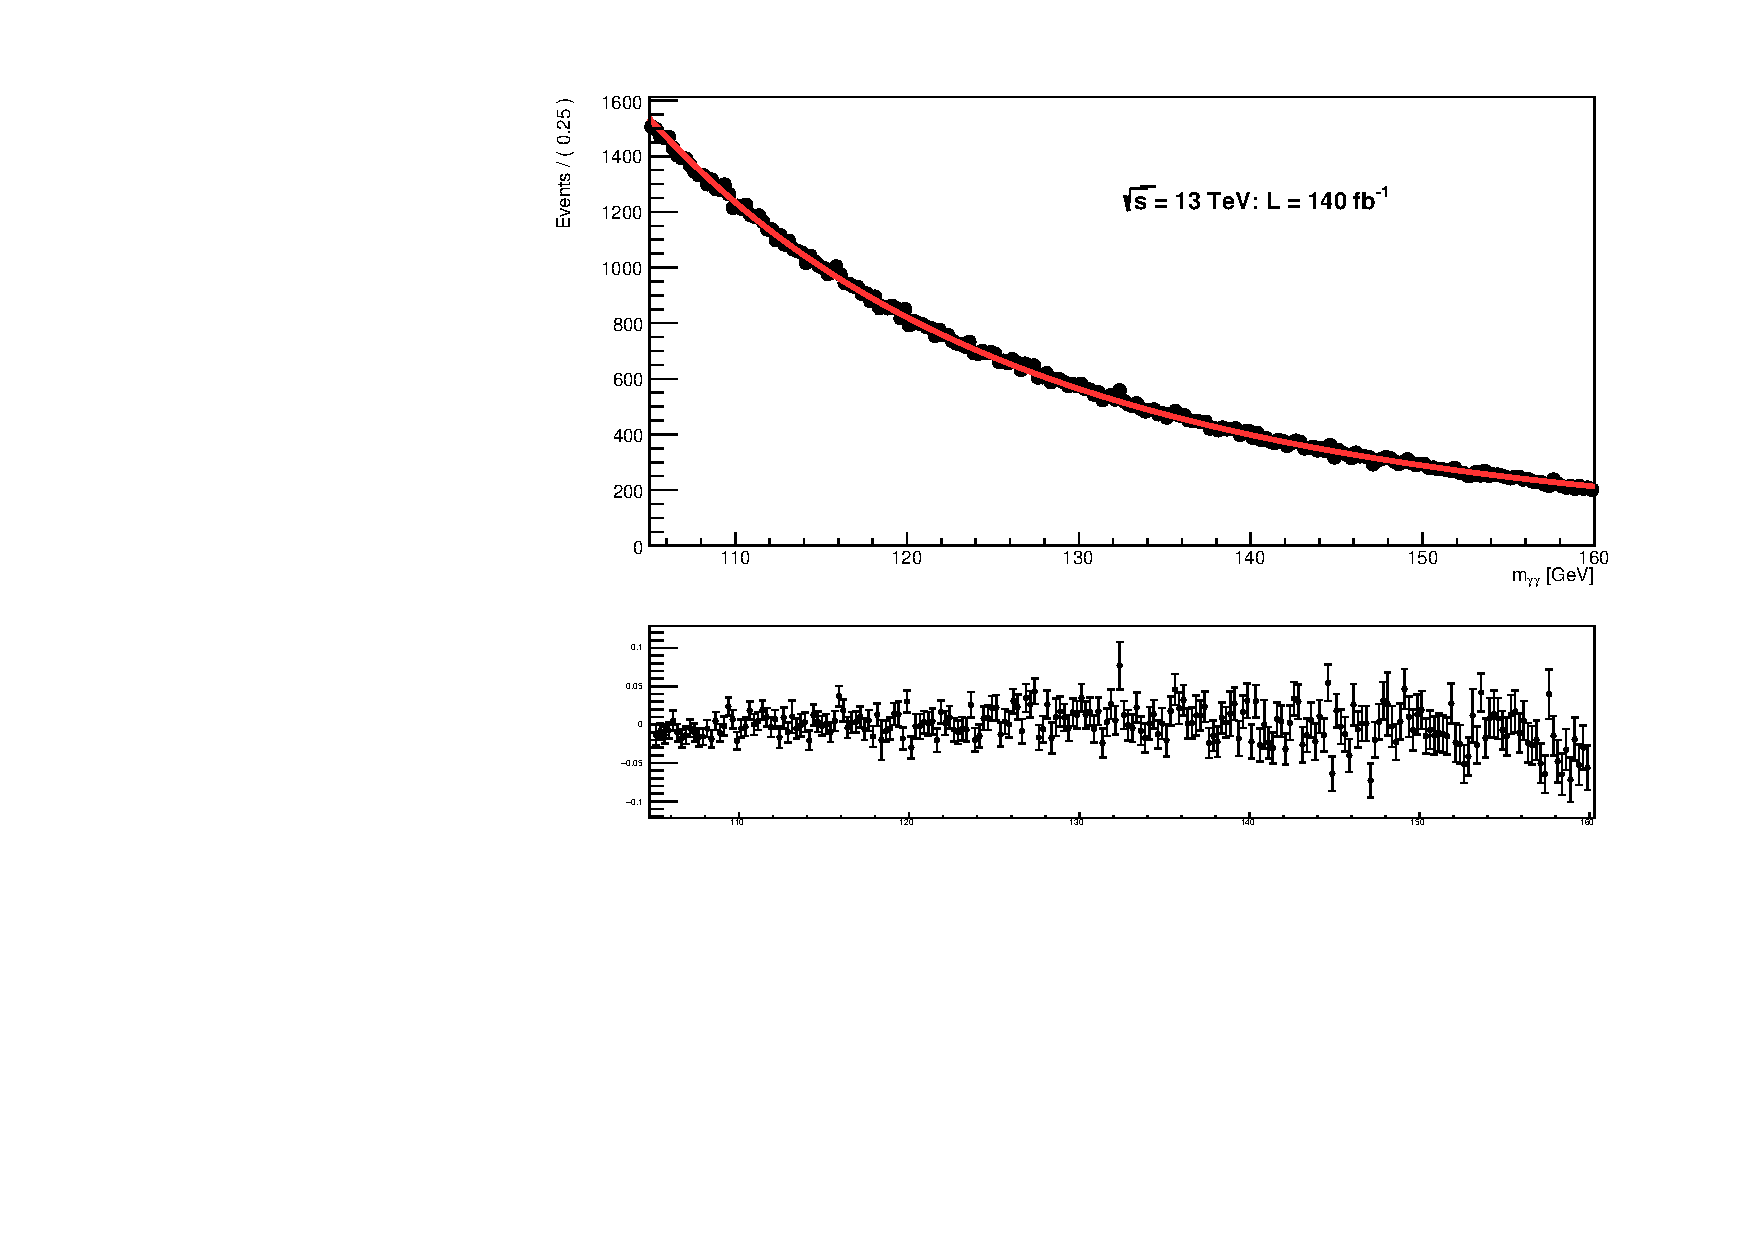
\includegraphics[scale=0.46]{fitPlot_pT_yy_bin_3_pow.pdf}
\caption{Example of fitting process for the background dataset in the mass range $105 \text{GeV} < m_{\gamma\gamma} < 160 \text{GeV}$ performed using the parametrization function with the minimum spurious signal (Pow) in the $pT_{\gamma\gamma}$ bin with best resolution ($10 \text{GeV} < p_T^{\gamma\gamma} < 15 \text{GeV}$).}
\label{bkg_example}
\end{figure}

\subsection{Spurious signal}
\label{spur_sign_sec}
The spurious signal method is used to study the bias in the signal yield evaluation for each observable bin. This kind of analysis is performed by fitting a background-only MonteCarlo sample with a distribution including both signal and background. The background sample is made mixing the $\gamma\gamma$, $\gamma j$ components following a data-driven approach. The $\gamma\gamma$ component is derived from S{\scriptsize HERPA} MonteCarlo simulation, while the $\gamma j$ component is taken from a control region. The $jj$ component is ignored in the background composition since it is negligible respect to the others. In principle, a null signal yield is expected from the fit. The effective yield of the fitted signal si called \emph{Spurious Signal} $SS$.
\\
The spurious signal yield extracted in this way from the background-only template $SS$ and its statistical uncertainty $\Delta_{SS}$ are used in the background parameterisation functions selection.
\begin{figure}[b!]
\centering
\subfloat{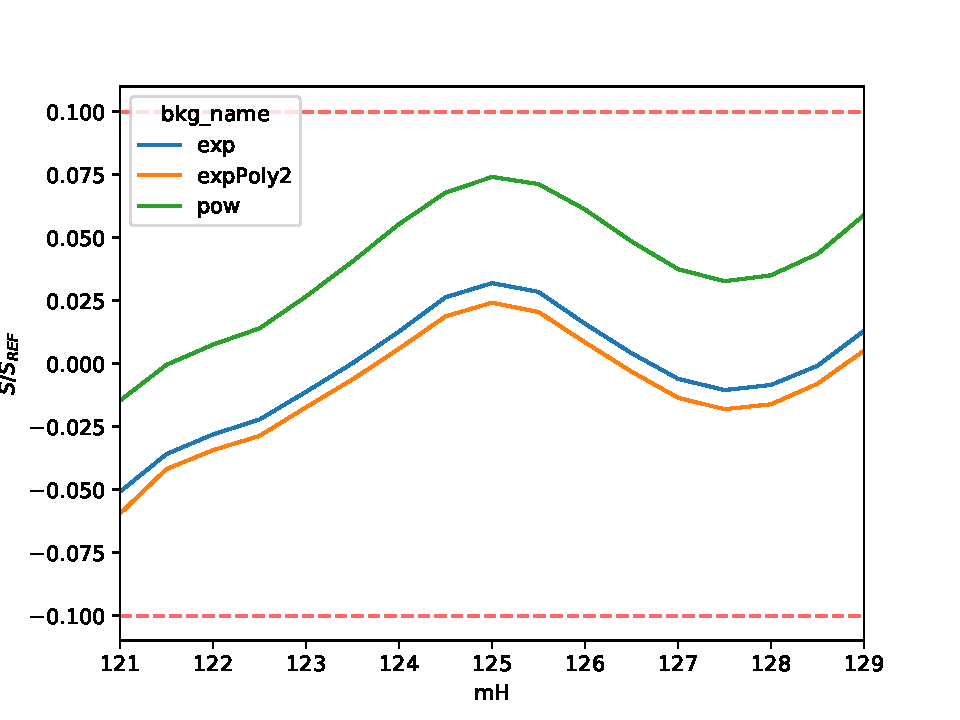
\includegraphics[scale=0.38]{total_Mu_pT_yy_bin_16.pdf}}
\subfloat{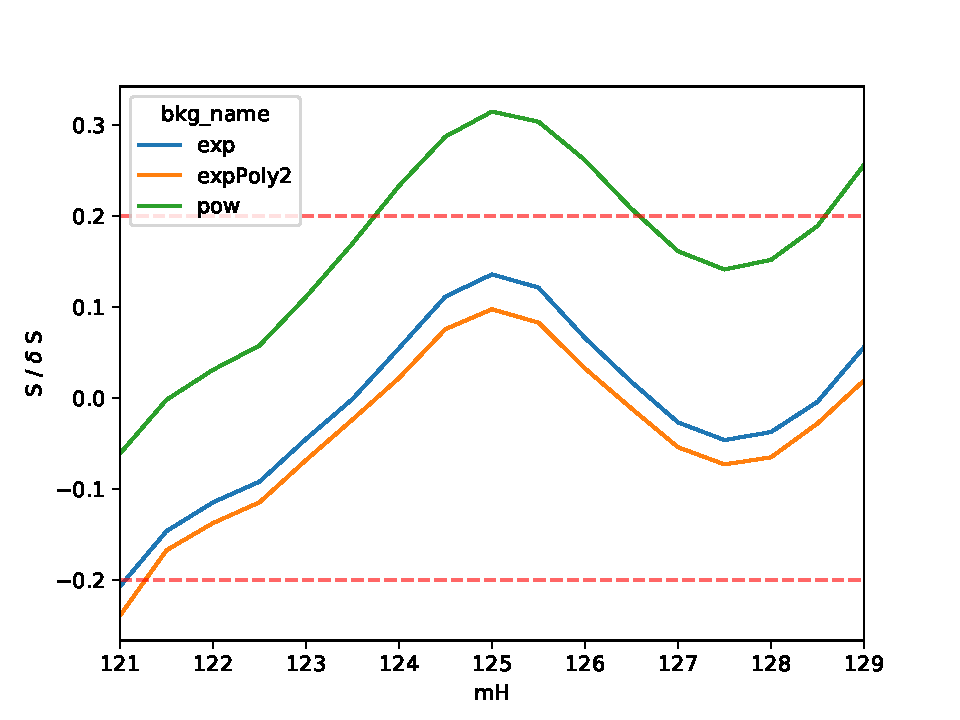
\includegraphics[scale=0.38]{total_Z_pT_yy_bin_16.pdf}} \\
\subfloat{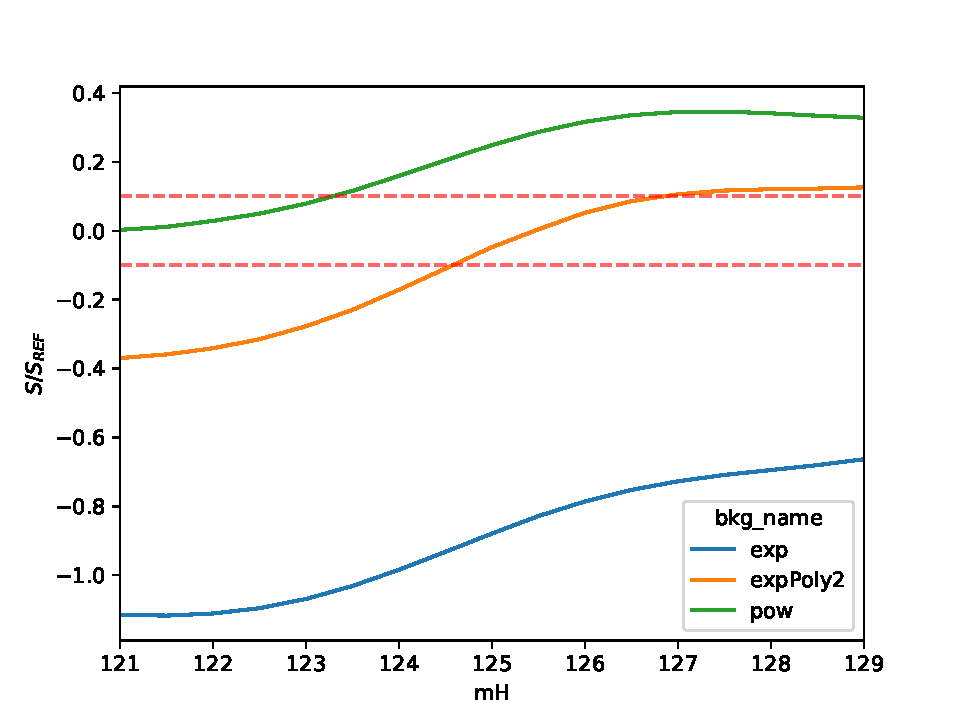
\includegraphics[scale=0.38]{total_Mu_pT_yy_bin_3.pdf}}
\subfloat{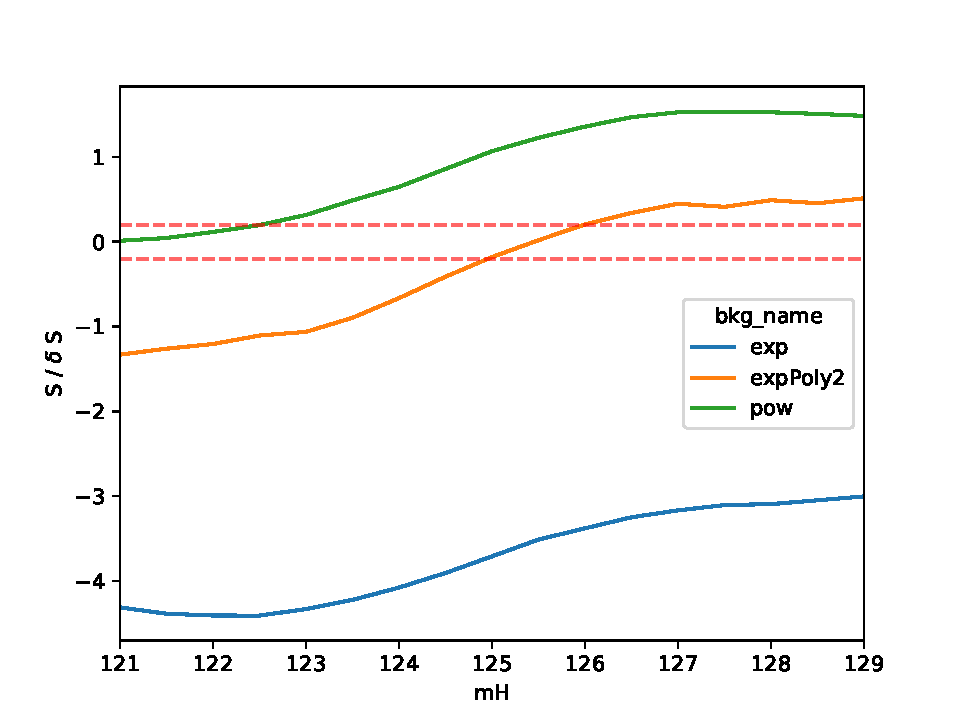
\includegraphics[scale=0.38]{total_Z_pT_yy_bin_3.pdf}} \\
\caption{Plots of $SS/S_{ref}$ and $SS/\Delta SS$ for $p_T^{\gamma\gamma}$ distribution in the best (upper plots for bin $16$) and worst (lower plots for bin $3$) bins. The dashed red lines show the selection conditions under which a functional form is selected ora rejected.}
\label{SS_example}
\end{figure}
\\The condition (Figure \ref{SS_example}) for a functional form to be accepted is that either
\begin{itemize}
\item $SS < 20 \%$ of the background uncertainty;
\item $SS < 10 \%$ of the number of expected signal events.
\end{itemize}
\begin{table}[h]
\centering
\small
\caption{Background templates and spurious signal results for the individual bins in $p_T^{\gamma\gamma}$ distribution.}
\label{SS}
\begin{tabular}{c | c | l r r r}
Bin & Range & Function & $|Max(SS)|$ & $SS/S_{ref} [\%]$ & $SS/\Delta SS [\%]$ \\
\hline
1 & $0 \text{GeV} < p_T^{\gamma\gamma} < 5 \text{GeV}$ & Pow & 37.4 & 13.6 & 38.4 \\
2 & $5 \text{GeV} < p_T^{\gamma\gamma} < 10 \text{GeV}$ & ExpPoly2 & 88.9 & 15.1 & 59.7 \\
3 & $10 \text{GeV} < p_T^{\gamma\gamma} < 15 \text{GeV}$ & Pow & 219.3 & 34.6 & 153.0 \\
4 & $15 \text{GeV} < p_T^{\gamma\gamma} < 20 \text{GeV}$ & ExpPoly2 & 67.5 & 11.6 & 40.3 \\
5 & $20 \text{GeV} < p_T^{\gamma\gamma} < 25 \text{GeV}$ & ExpPoly2 & 120.1 & 23.5 & 73.5 \\
6 & $25 \text{GeV} < p_T^{\gamma\gamma} < 30 \text{GeV}$ & ExpPoly2 & 25.9 & 5.9 & 20.6 \\
7 & $30 \text{GeV} < p_T^{\gamma\gamma} < 35 \text{GeV}$ & ExpPoly2 & 71.1 & 18.9 & 57.2 \\
8 & $35 \text{GeV} < p_T^{\gamma\gamma} < 45 \text{GeV}$ & ExpPoly2 & 61.6 & 10.3 & 38.6 \\
9 & $45 \text{GeV} < p_T^{\gamma\gamma} < 60 \text{GeV}$ & ExpPoly2 & 82.1 & 13.1 & 59.7 \\
10 & $60 \text{GeV} < p_T^{\gamma\gamma} < 80 \text{GeV}$ & Exp & 27.6 & 5.3 & 21.6 \\
11 & $80 \text{GeV} < p_T^{\gamma\gamma} < 100 \text{GeV}$ & ExpPoly2 & 59.1 & 18.2 & 62.8 \\
12 & $100 \text{GeV} < p_T^{\gamma\gamma} < 120 \text{GeV}$ & ExpPoly2 & 47.6 & 22.7 & 74.2 \\
13 & $120 \text{GeV} < p_T^{\gamma\gamma} < 140 \text{GeV}$ & ExpPoly2 & 13.1 & 9.0 & 29.3 \\
14 & $140 \text{GeV} < p_T^{\gamma\gamma} < 170 \text{GeV}$ & Pow & 23.3 & 16.1 & 64.1 \\
15 & $170 \text{GeV} < p_T^{\gamma\gamma} < 200 \text{GeV}$ & Pow & 15.3 & 17.3 & 65.9 \\
16 & $200 \text{GeV} < p_T^{\gamma\gamma} < 250 \text{GeV}$ & Exp & 4.0 & 5.0 & 20.4 \\
17 & $250 \text{GeV} < p_T^{\gamma\gamma} < 350 \text{GeV}$ & Pow & 4.5 & 8.0 & 33.3 \\
18 & $p_T^{\gamma\gamma} \geq 350 \text{GeV}$ & Pow & 5.8 & 26.1 & 93.5
\end{tabular}
\end{table}
In the case of none of the functions is selected, the selection criteria is based on the choice of the functional form which has the minimum value for the spurious signal, in order to find the function which best describes the background spectrum.
\\
In Table \ref{SS} the selected best background parameterisations for $p_T^{\gamma\gamma}$ distribution and relative spurious signals are summarized . The selected background functions for other observables are presented in Appendix \ref{CB_parameters_appendix}.
\\
For each bin of the observable's distribution, the selected function is given, followed by the maximal spurious signal value $|Max(SS)|$ and the spurious signal uncertainty $SS/S_{ref}$ for that function in the single bin. The spurious signal uncertainty is evaluated as the ratio between the maximal spurious signal value and the reference signal based on MonteCarlo simulations.

\section{Unfolding}
In any experimental analysis, the distribution of every observable is distorted and biased due to experimental limitations effects, as the limited acceptance, the reconstruction efficiency and the finite resolution. The unfolding is the procedure to correct a measured quantity estimating the \emph{truth-level} spectrum, once the \emph{reco-level} distribution is known.
\\
Through the unfolding procedure it is possible to obtain results independent of detector and reconstruction effects, making in this way the unfolded differential distributions easily comparable among different experiments and with the theoretical predictions too \cite{refId0}.
\\\\
In this work, two different unfolding methods are tested, in order to obtain the best corrections to be applied at the measured differential cross sections, so they can be unfolded to particle level cross sections and in this way compared to the theoretical Standard Model predictions:
\begin{itemize}
\item the \emph{bin-by-bin} unfolding method;
\item the \emph{inverse-matrix} unfolding method.
\end{itemize}
The theoretical predictions used are the ones provided by the MonteCarlo simulations described in Section \ref{mc_sim}.

\subsection{The bin-by-bin unfolding method}
\label{c_factors_sec}
The bin-by-bin method corrects the reconstructed events with the true number of events (Figure \ref{true/reco}) with just a multiplicative factor for each bin, called \emph{c factor}.
\\
Consider $N_i^{\text{reco, peak}}$ as the expected reconstructed signal yield under the resonant peak (e.g. the Crystal Ball function) in a given reconstructed category. This quantity can be derived from the expected signal yield at particle level in the corresponding fiducial bin $N_i^\text{true, $\gamma\gamma$, fid}$ through the relation
\begin{equation}
N^\text{reco, peak}_i = \underbrace{L \sigma_i^\text{fid} Br_{\gamma\gamma}}_{N_i^\text{true, $\gamma\gamma$, fid}} \cdot C_i
\end{equation}
simply scaling $N_i^{\text{true, }\gamma\gamma \text{, fid}}$, the number of signal events at particle level in the fiducial region, by the correction factor $C_i$, shown for each distribution in Table \ref{c_factors_table}. These factors are computed from MonteCarlo simulations as the ratio of the number of signal events expected to pass the detector level criteria and the number of events expected to pass the corresponding particle level criteria
\begin{equation}
C_i = \left(\frac{N^\text{reco, peak}_i}{N_i^\text{true, $\gamma\gamma$, fid}}\right)_\text{MC}
\end{equation}
where the number of expected events at both detector reconstructed and particle level are computed from MonteCarlo simulations considering all the production modes.
\begin{figure}[b!]
\centering
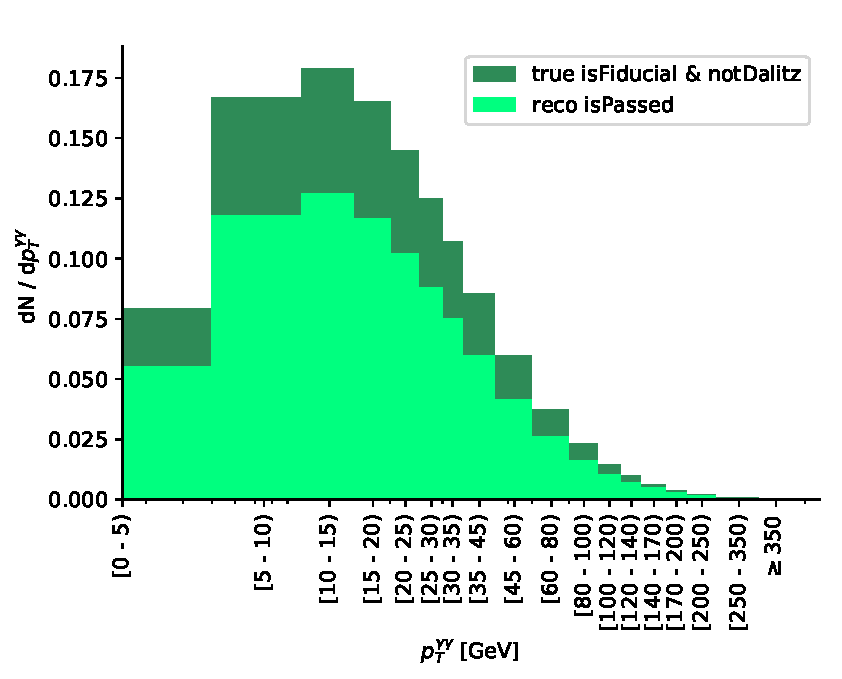
\includegraphics[scale=0.6]{reco-true_comparison/comparison_true_reco_pT_yy_for_c_factors.pdf}
\caption{Comparison of the $p_T^{\gamma\gamma}$ distribution at reco level for events passing the particle level criteria and for events passing the corresponding detector reconstructed level criteria, computed by using MonteCarlo simulation.}
\label{true/reco}
\end{figure}
\begin{table}[h]
\centering
\small
\caption{Bin-by-bin correction factors for each bin of all observables' distributions.}
\label{c_factors_table}
\begin{tabular}{l | rrrrrr}
Bin &  $p_T^{\gamma\gamma}$ & $|y|_{\gamma\gamma}$ & $p_T^{j1, 30}$ & $\Delta\phi_{jj}^{30}$ & $N_j^{30}$ & $m_{jj}^{30}$ \\
\hline
0 &					- & 				- & 				0.64 & 					0.68 & 			- & 			0.68 \\ 
1 &                  0.69 &                 0.72 &           0.84 &                   0.82 &       0.65 &          0.87 \\
2  &                  0.71 &                 0.72 &           0.71 &                   0.86 &       0.76 &           0.8 \\
3  &                  0.71 &                 0.72 &           0.72 &                   0.86 &        0.8 &          0.85 \\
4  &                  0.71 &                 0.72 &           0.75 &                   0.82 &       0.95 &           0.9 \\
5  &                  0.71 &                 0.72 &           0.77 &                      - &          - &             - \\
6  &                  0.71 &                 0.72 &           0.76 &                      - &          - &             - \\
7  &                  0.70 &                  0.70 &              - &                      - &          - &             - \\
8  &                  0.70 &                 0.69 &              - &                      - &          - &             - \\
9  &                  0.70 &                 0.68 &              - &                      - &          - &             - \\
10 &                  0.70 &                    - &              - &                      - &          - &             - \\
11 &                  0.70 &                    - &              - &                      - &          - &             - \\
12 &                  0.72 &                    - &              - &                      - &          - &             - \\
13 &                  0.73 &                    - &              - &                      - &          - &             - \\
14 &                  0.75 &                    - &              - &                      - &          - &             - \\
15 &                  0.76 &                    - &              - &                      - &          - &             - \\
16 &                  0.77 &                    - &              - &                      - &          - &             - \\
17 &                  0.79 &                    - &              - &                      - &          - &             - \\
18 &                  0.80 &                    - &              - &                      - &          - &             - 
\end{tabular}
\end{table}
\\The $N^\text{reco, peak}_i$ expected yields must take into account both $H \rightarrow \gamma\gamma$ (fiducial and not fiducial) and the $H \rightarrow \gamma\gamma *$ resonant processes, the latter generally known as Dalitz processes, which cannot be distinguished at detector reconstructed level, while $N^\text{true, $\gamma\gamma$, fid}_i$ is computed only for $H \rightarrow \gamma\gamma$
\begin{align}
N^\text{reco, peak}_i &= N^\text{reco, peak, $\gamma\gamma$}_i + N^\text{reco, peak, $\gamma\gamma^*$}_i \\
&= \sum_{S\in\text{samples}} L_S \sigma_S Br_{\gamma\gamma} P(\text{pass}, i|S, \gamma\gamma) + (\gamma\gamma\leftrightarrow\gamma\gamma^*) \\
&= \sum_{S\in\text{samples}} L_S \sigma_S Br_{\gamma\gamma} \left(\frac{ \sum_{n\in\text{pass, i, $\gamma\gamma$}} w^\text{final}_{n} } { \sum_{n\in\gamma\gamma} w^\text{initial}_{n} }\right)_S + (\gamma\gamma\leftrightarrow\gamma\gamma^*)
\end{align}
\begin{align}
N^\text{true, $\gamma\gamma$, fid}_i
&= \sum_{S\in\text{samples}} L_S \sigma_S Br_{\gamma\gamma} \underbrace{P(\text{true-fid-$i$}|S, \gamma\gamma)}_{A_{S, i}}\\
&= \sum_{S\in\text{samples}} L_S \sigma_S Br_{\gamma\gamma} \left(\frac{ \sum_{n\in\text{i, $\gamma\gamma$}} w^\text{initial}_{n} } { \sum_{n\in\gamma\gamma} w^\text{initial}_{n} }\right)_S
\end{align}
where the $P(\text{pass}, i|S, \gamma\gamma)$ is the probability for a reconstructed event to pass the selection criteria, computed as the the ratio between the number of events passing the selection and the total number of events at particle level for a given sample, while $P(\text{true-fid-$i$}|S, \gamma\gamma)$, generally known as the acceptance $A_{S, i}$, is the probability for a particle level event to fall in the fiducial phase space for a given sample. The summations are done over all the samples, for each production mode and different period.

\subsection{The inverse-matrix unfolding method}
\label{matrix_sec}
Differently from the bin-by-bin unfolding method, in the inverse matrix unfolding method the migrations and correlations between bins in the detector reconstruction are explicitely modelled. The matrix considered here is the signal efficiency matrix which describes both the efficiency and the migration effects \cite{article_matrix_method}. Some care should be taken to take into account resonant events which are not signal: Dalitz $H \rightarrow \gamma\gamma *$ and out of fiducial $H \rightarrow \gamma\gamma$ events.
\\\\
In case of infinite detector resolution and no other biasing effects, the detector response matrix is just a diagonal matrix, where for each reconstructed bin is associated only the corresponding bin at particle level. In a normal experiment, though, experimental limitation effects leads to events' migrations passing from particle level to the detector reconstructed ones, corrected by the coefficients turning out from the inverse detector response matrix.
\\\\
Considering the number of expected selected events under the resonant peak $N^\text{reco, peak}_R$, in the detector reconstructed category $R$, it can be decomposed in the two components for the $H \rightarrow \gamma\gamma$ and $H \rightarrow \gamma\gamma *$ processes
\begin{align}
N^\text{reco, peak}_R &= N^\text{reco, peak, $\gamma\gamma$}_R + N^\text{reco, peak, $\gamma\gamma^*$}_R \\
&= \sum_{T\neq \gamma\gamma^*} N^\text{reco, peak}_{R,T} + N^\text{reco, peak}_{R, \gamma\gamma^*} \\
&= \sum_{T\neq \gamma\gamma^*} N_{T}\mathlarger{\varepsilon}(R|T) + N_{T=\gamma\gamma*}\mathlarger{\varepsilon}(R|\gamma\gamma^*) \\
&= \sum_{T\neq \gamma\gamma^*} L \sigma_T Br_{\gamma\gamma} \mathlarger{\varepsilon}(R|T) + L\underbrace{\left(\sum_{T\neq\gamma\gamma*}\sigma_\text{T}\right)}_{\sigma^\text{tot}} Br_{\gamma\gamma^*} \mathlarger{\varepsilon}(R|\gamma\gamma^*)
\end{align}
\phantom{i}\hspace{0.5cm}$R = $ (reco pass bin1), (reco pass bin2), \ldots,
\\
\phantom{i}\hspace{0.5cm}$T = $ ($\gamma\gamma$ fiducial bin1), ($\gamma\gamma$ fiducial bin2), \ldots, ($\gamma\gamma$ not-fiducial), ($\underbrace{\gamma\gamma^*}_\text{Dalitz}$)
\\
where $N^\text{reco, peak}_R$ are the expected number of events reconstructed in bin $R$ coming from the bin $T$, while $N_T$ is the number of events generated in the true bin $T$.
\\\\
The efficiency matrix $\mathlarger{\varepsilon}(R|T)$, generally known as \emph{folding matrix} and deriving from the yield matrix in Figure \ref{yield_matrix}, is evaluated from MonteCarlo simulations and represents the probability for a given particle-level $T$ event to be reconstructed as a given detector reconstructed $R$ event
\begin{equation}
\mathlarger{\varepsilon}(R|T) = P[R|T] = \left(\frac{N_{R, T}}{N_T}\right)_\text{MC}
\end{equation}
In the case of Dalitz $H \rightarrow \gamma\gamma *$ events, the Branching Ratio $Br_{\gamma\gamma^*}$ is derived from the $H \rightarrow \gamma\gamma$ Branching Ratio $Br_{\gamma\gamma}$, rescaled by the fraction of Dalitz events in the MonteCarlo dataset
\begin{equation}
Br_{\gamma\gamma*} = Br_{\gamma\gamma}\times\left( \frac{N_{\gamma\gamma^*}}{N_{\gamma\gamma}}\right)_\text{MC}
\end{equation}
while the out of fiducial cross sections $\sigma_\text{$\gamma\gamma$, not-fiducial}$, being those impossible to be reconstructed at detector level due to the finite detecting acceptance, are taken rescaling the total cross section $\sigma_\text{tot}$ by the acceptance of the detector $A_\text{not-fiducial}$
\begin{equation}
\sigma_\text{$\gamma\gamma$, not-fiducial} = \sigma^\text{tot} \times A_\text{not-fiducial} =\underbrace{\left(\sum_{T\neq\gamma\gamma^*, \text{non-fid}}\sigma_T\right)}_{\sigma^\text{fid}}\times\frac{A_\text{not-fiducial}}{1-A_\text{not-fiducial}}
\end{equation}
with
\begin{equation}
A_\text{not-fiducial}=\left(\frac{N_\text{$\gamma\gamma$, not-fiducial}}{N_{\gamma\gamma}}\right)_\text{MC}
\end{equation}
With respect to the analysis published by ATLAS \cite{ATLAS-CONF-2018-018}, the different and original approach of this work consists in considering the Dalitz and the out of fiducial phase space events in separate and distinct categories, in order to improve the accuracy of the unfolding method.
\\
As an example, in Figure \ref{pT_yy_migration} the migration matrix for $p_T^{\gamma\gamma}$ distribution is shown. It can be seen how, as growing values of $p_T^{\gamma\gamma}$, the migration contributions get smaller due to improving of the detector resolution. In the first two rows the separated Dalitz and out of fiducial phase space categories are displayed. Thanks to the design of the selection cut, the contribution from non-fiducial region and Dalitz events is very small.
\begin{figure}[H]
\centering
\subfloat[][]{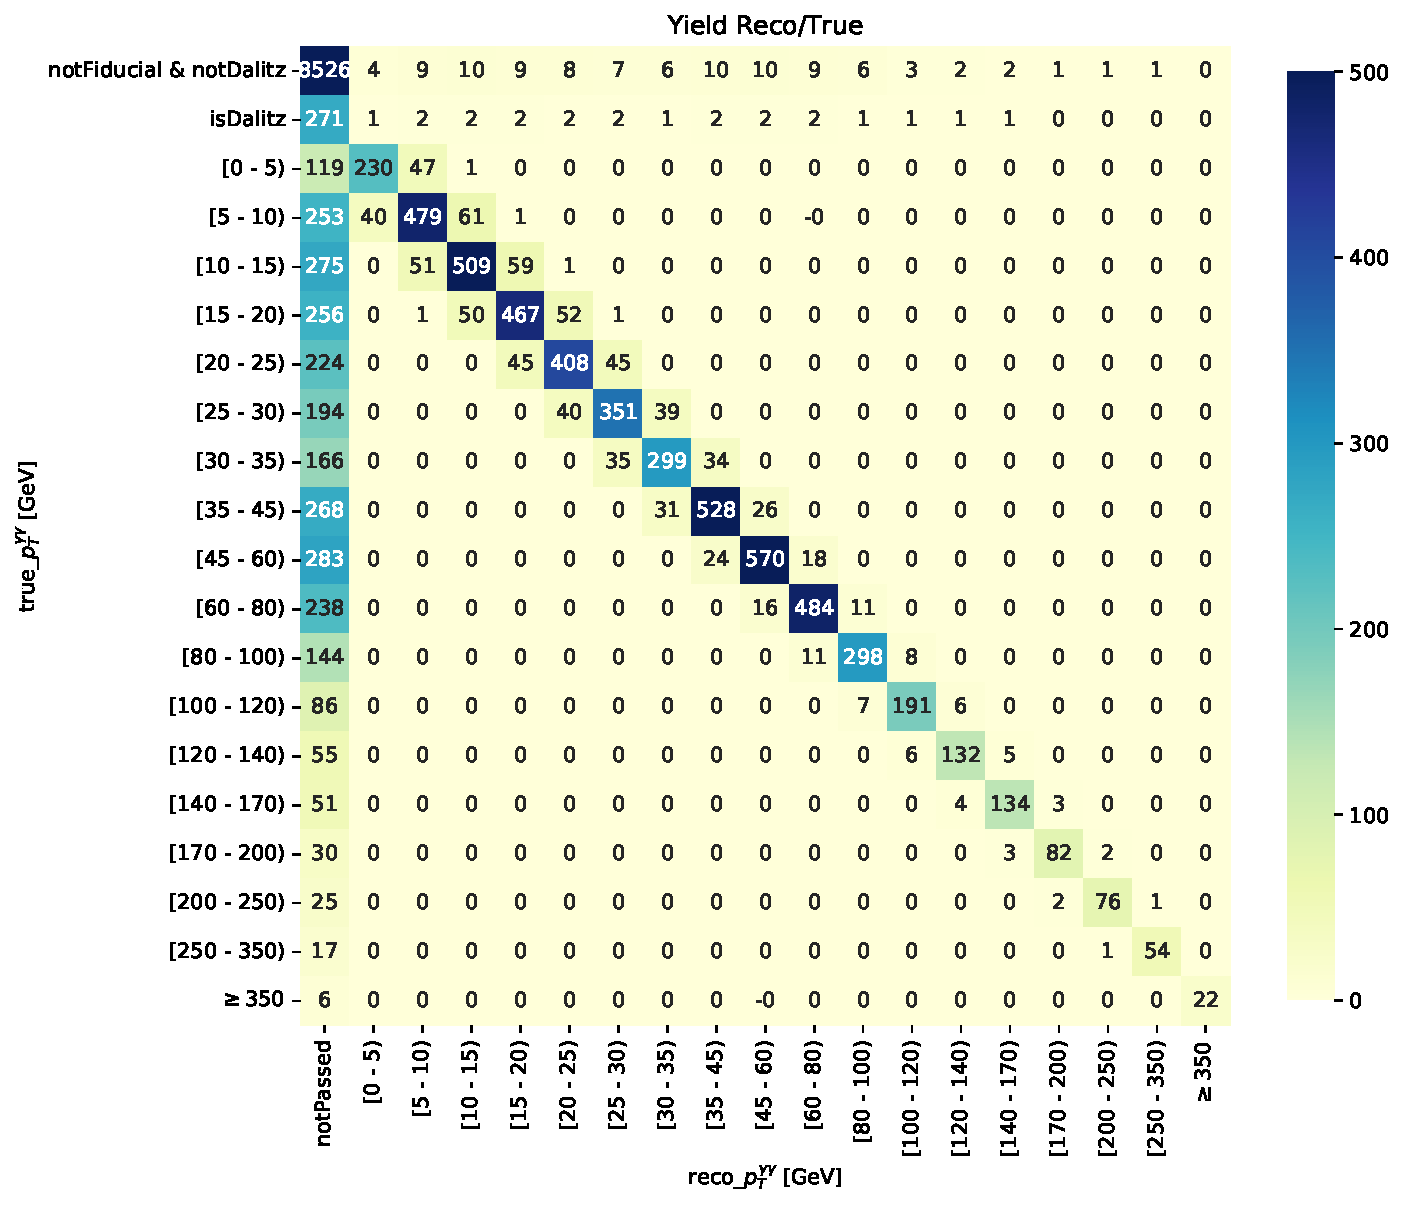
\includegraphics[scale=0.44]{folding_matrices/yield_reco_true_All_pT_yy_mcAll_prodAll_sysNominal_LUMI_138972.pdf}
\label{yield_matrix}} \\
\subfloat[][]{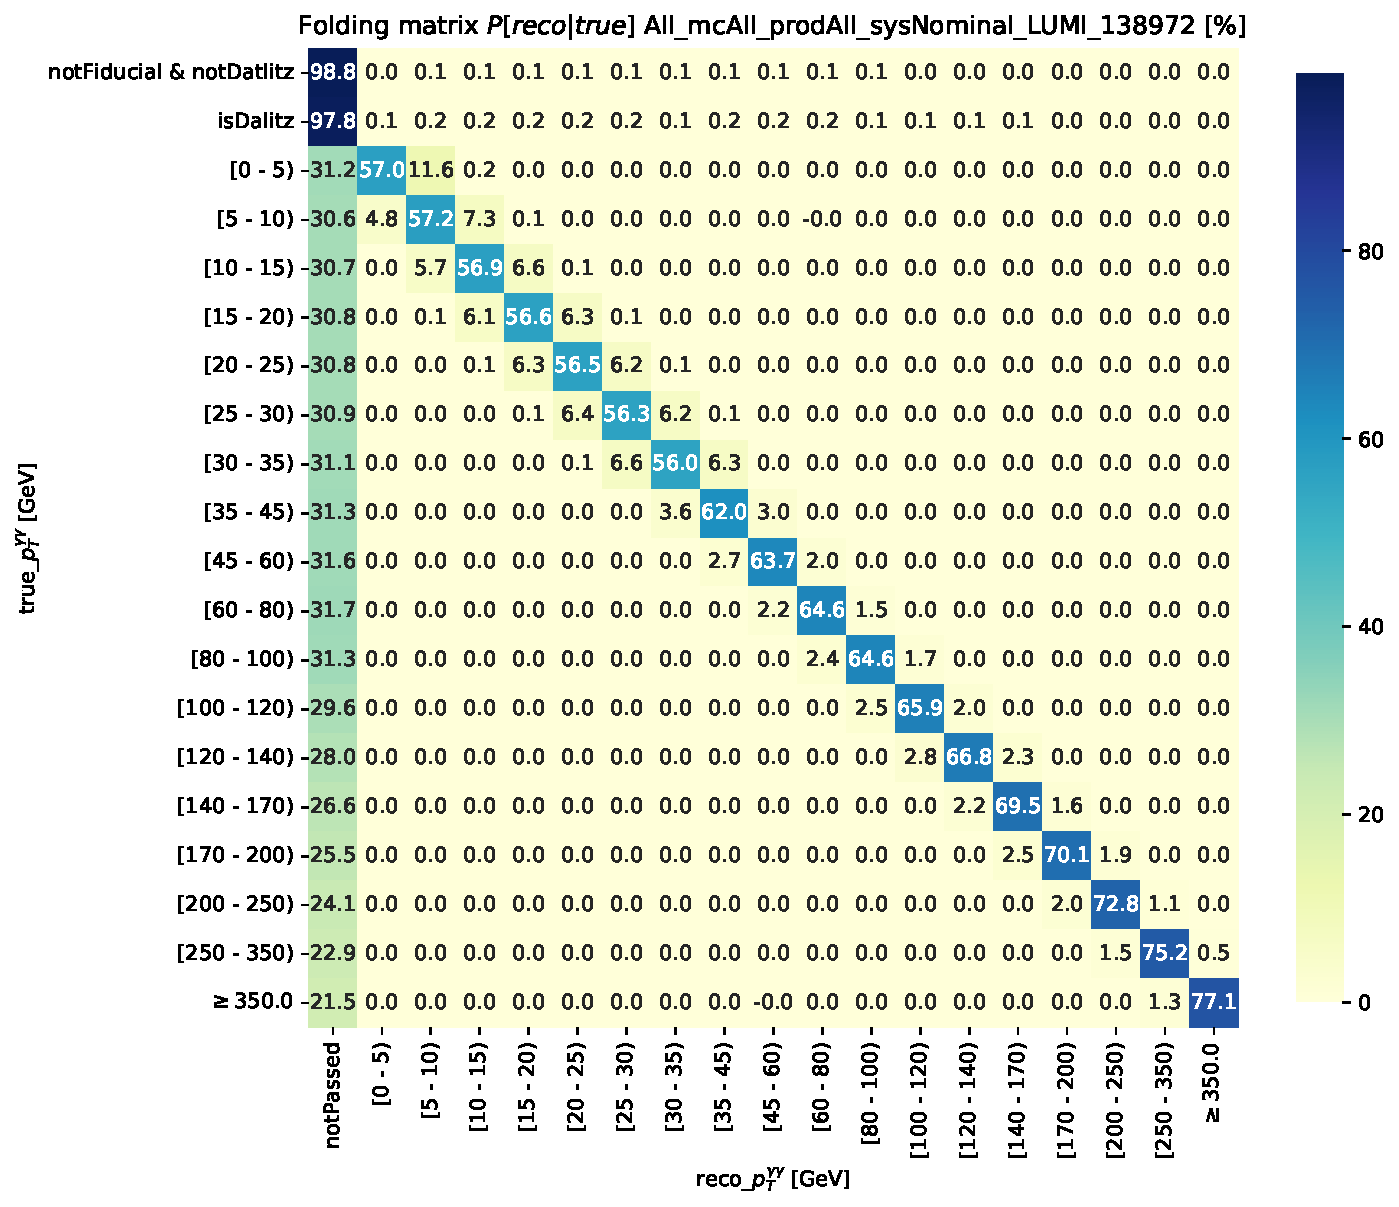
\includegraphics[scale=0.44]{folding_matrices/folding_matrix_P_reco_true_All_pT_yy_mcAll_prodAll_sysNominal_LUMI_138972.pdf}
\label{pT_yy_migration}}
\caption{a)Expected yield for each reconstructed and true bin, normalized to $140$ fb$^{-1}$; b)Migration matrix for $p_T^{\gamma\gamma}$ distribution using the dataset normalized to $140$ fb$^{-1}$. The notPassed bins are not used in the analysis.}
\end{figure}

\section{Statistical model}
The fiducial differential cross sections are extracted performing a simultaneous fit on the  $m_{\gamma\gamma}$ distribution over every bin of each observable. A PDF combines the signal Double-Sided Crystal Ball parameterisation and the background for the considered bin. The observed values are derived fitting data, while the expected ones are obtained through a fit from Asimov dataset. The likelihood function is defined as in Eq.(\ref{likelihood})
\begin{equation}
\mathcal{L}_R(m_{\gamma\gamma}; \vec{\sigma}, N_{\text{bkg}}, \vec{\theta}) = \frac{e^{-\nu}}{n!} \prod_{j}^{n}\Bigl[N_R^{\text{Reco, peak}}(\vec{\sigma}, \vec{\theta}) \mathcal{S}(m_{\gamma\gamma}^j; \vec{\theta}) + N_{\text{bkg}, R} \mathcal{B}_R(m_{\gamma\gamma}^j)\Bigr]
\label{likelihood}
\end{equation} 
\begin{table}[h]
\centering
\tiny
\caption{Energy scale systematics $\sigma_{ES}$ on the left and energy resolution systematics on the right, expressed in \%, for each observable in the analysis.}
\label{ES_ER_table}
\begin{tabular}{l | cccccc}
Bin & $p_T^{\gamma\gamma}$ & $|y|_{\gamma\gamma}$ & $p_T^{j1}$ & $\Delta\phi_{jj}^{30}$ & $N_j^{30}$ & $m_{jj}^{30}$ \\
\hline
0 & - & - & 0.43 & 0.43 & - & 0.43 \\
1 & 0.42 & 0.27 & 0.44 & 0.46 & 0.43 & 0.48 \\
2 & 0.42 & 0.28 & 0.47 & 0.51 & 0.45 & 0.49 \\
3 & 0.42 & 0.30 & 0.49 & 0.51 & 0.48 & 0.49 \\
4 & 0.42 & 0.34 & 0.54 & 0.46 & 0.51 & 0.50 \\
5 & 0.42 & 0.38 & 0.54 & - & - & - \\
6 & 0.42 & 0.44 & 0.63 & - & - & - \\
7 & 0.43 & 0.53 & - & - & - & - \\
8 & 0.43 & 0.60 & - & - & - & - \\
9 & 0.44 & 0.66 & - & - & - & - \\
10 & 0.46 & - & - & - & - & - \\
11 & 0.47 & - & - & - & - & - \\
12 & 0.48 & - & - & - & - & - \\
13 & 0.50 & - & - & - & - & - \\
14 & 0.53 & - & - & - & - & - \\
15 & 0.55 & - & - & - & - & - \\
16 & 0.58 & - & - & - & - & - \\
17 & 0.62 & - & - & - & - & - \\
18 & 0.65 & - & - & - & - & - \\
\end{tabular} \qquad
\begin{tabular}{l | cccccc}
Bin & $p_T^{\gamma\gamma}$ & $|y|_{\gamma\gamma}$ & $p_T^{j1}$ & $\Delta\phi_{jj}^{30}$ & $N_j^{30}$ & $m_{jj}^{30}$ \\
\hline
0 & - & - & 6.8 & 7.0 & - & 7.0 \\ 
1 & 6.6 & 5.4 & 7.2 & 7.8 & 6.8 & 8.4 \\
2 & 6.5 & 5.4 & 7.8 & 9.2 & 7.5 & 8.6 \\
3 & 6.5 & 5.6 & 8.6 & 9.4 & 8.3 & 8.9 \\
4 & 6.5 & 5.8 & 10.7 & 8.0 & 9.1 & 8.3 \\
5 & 6.5 & 6.1 & 10.7 & - & - & - \\
6 & 6.6 & 6.5 & 16.5 & - & - & - \\
7 & 6.7 & 7.0 & - & - & - & - \\
8 & 6.9 & 8.4 & - & - & - & - \\
9 & 7.0 & 10.8 & - & - & - & - \\
10 & 7.1 & - & - & - & - & - \\
11 & 7.7 & - & - & - & - & - \\
12 & 7.9 & - & - & - & - & - \\
13 & 8.4 & - & - & - & - & - \\
14 & 10.6 & - & - & - & - & - \\
15 & 11.1 & - & - & - & - & - \\
16 & 12.4 & - & - & - & - & - \\
17 & 14.5 & - & - & - & - & - \\
18 & 18.0 & - & - & - & - & - \\
\end{tabular}
\end{table}
\\In Eq.(\ref{likelihood}) many ingredients are recognisable: $m_{\gamma\gamma}^j$ is the diphoton invariant mass for the event $j$, $\mathcal{S}(m_{\gamma\gamma}^j; \theta_k)$ and $\mathcal{B}(m_{\gamma\gamma}^j)$ are the signal and background probability distribution functions respectively and $N_R^{\text{Reco, peak}}(\vec{\sigma}, \vec{\theta})$ represents the total expected signal yield under the resonant peak and $N_{\text{bkg}, R}$ is the expected number of background events for the considered reconstructed category.
\\
The systematics are introduced inserting degrees of freedom which can modify specific quantities. As an example, the energy scale systematic is implemented as a shift of the peak of the Double-Side Crystal Ball signal function $\sigma_{CB} \rightarrow \sigma_{CB}(1+\sigma_{ES}\theta_{ES})$ where $\sigma_{ES}$ is the effect of the energy scale systematic on the Crystal Ball peak, while $\theta_{ES}$ is the nuisance parameter constrained with a Gaussian distribution $G[0;\theta_{ES}, 1]$.
\\
The product of the likelihood for each bin is multiplied by the product of the Gaussian constrains
\begin{equation}
\prod_{k} G_k(\theta_k; 0, 1)
\end{equation}
Most of the nuisance parameters are correlated across all bins in a given distribution.
\\
All of the other systematics are implemented in the likelihood in a similar way.
\\
Table in \ref{ES_ER_table} on the left shows the effect of the energy systematic on $\sigma_{CB}$, while table  in \ref{ES_ER_table} on the right shows the effect of the energy resolution systematic on $\mu_{CB}$.
\\
Some nuisance parameters are not constrained. For example, the yield and shape of the background parameter are free and determined from the mass sidebands.
\\\\
Systematic effects are evaluated re-running the analysis (e.g. signal parametrisation, signal efficiencies) on samples with systematic effects applied.
\\
In the previous ATLAS published papers the analysis was split in two separate steps. First, the signal yield is extracted, then the unfolding procedure was applied. In this work the two steps are done together in the likelihood optimization.

\section{Expected results}
The expected results for the fiducial differential cross sections multiplied for the Branching Ratio for the $H \rightarrow \gamma\gamma$ decay channel are obtained fitting the Asimov dataset\footnote{The Asimov dataset is a dataset generated from the pdf using nominal values from the signal and values from the background evaluated fitting the data sidebands.}.
The results are compared to the Standard Model predictions for the separate differential variables distributions. Both bin-by-bin unfolding method and matrix unfolding method has been used in the analysis.
\begin{figure}[htb]
\centering
\includegraphics[scale=0.4]{plot-correlation/binbybin/pT_yy/correlation_pT_yy_AsimovSB.pdf}
\caption{Correlation matrix in \% of the fitted cross sections' categories for $p_T^{\gamma\gamma}$, using the bin-by-bin unfolding method.It is easy to see how the bins are almost uncorrelated, as expected.}
\label{correlation_bin-by-bin_unfolding}
\end{figure}
\\Differential cross-sections results for analysis performed using both unfolding methods are shown down below. The correlation matrices for the distribution categories show the differences between the two unfolding methods.
\\\\
Using the bin-by-bin unfolding, the categories are uncorrelated because there are no modelling of the migrations from one category to another and, in fact, the correlation matrix is almost diagonal, as an example in Figure \ref{correlation_bin-by-bin_unfolding}.
\\\\
Differently from the bin-by-bin unfolding, using the matrix unfolding the categories are correlated because of the migrations from bin to bin. In this case, in fact, the correlation matrix shows some correlations between the diagonal neighbouring categories, as it is shown in Figure \ref{correlation_matrix_unfolding}.
\begin{figure}[t]
\centering
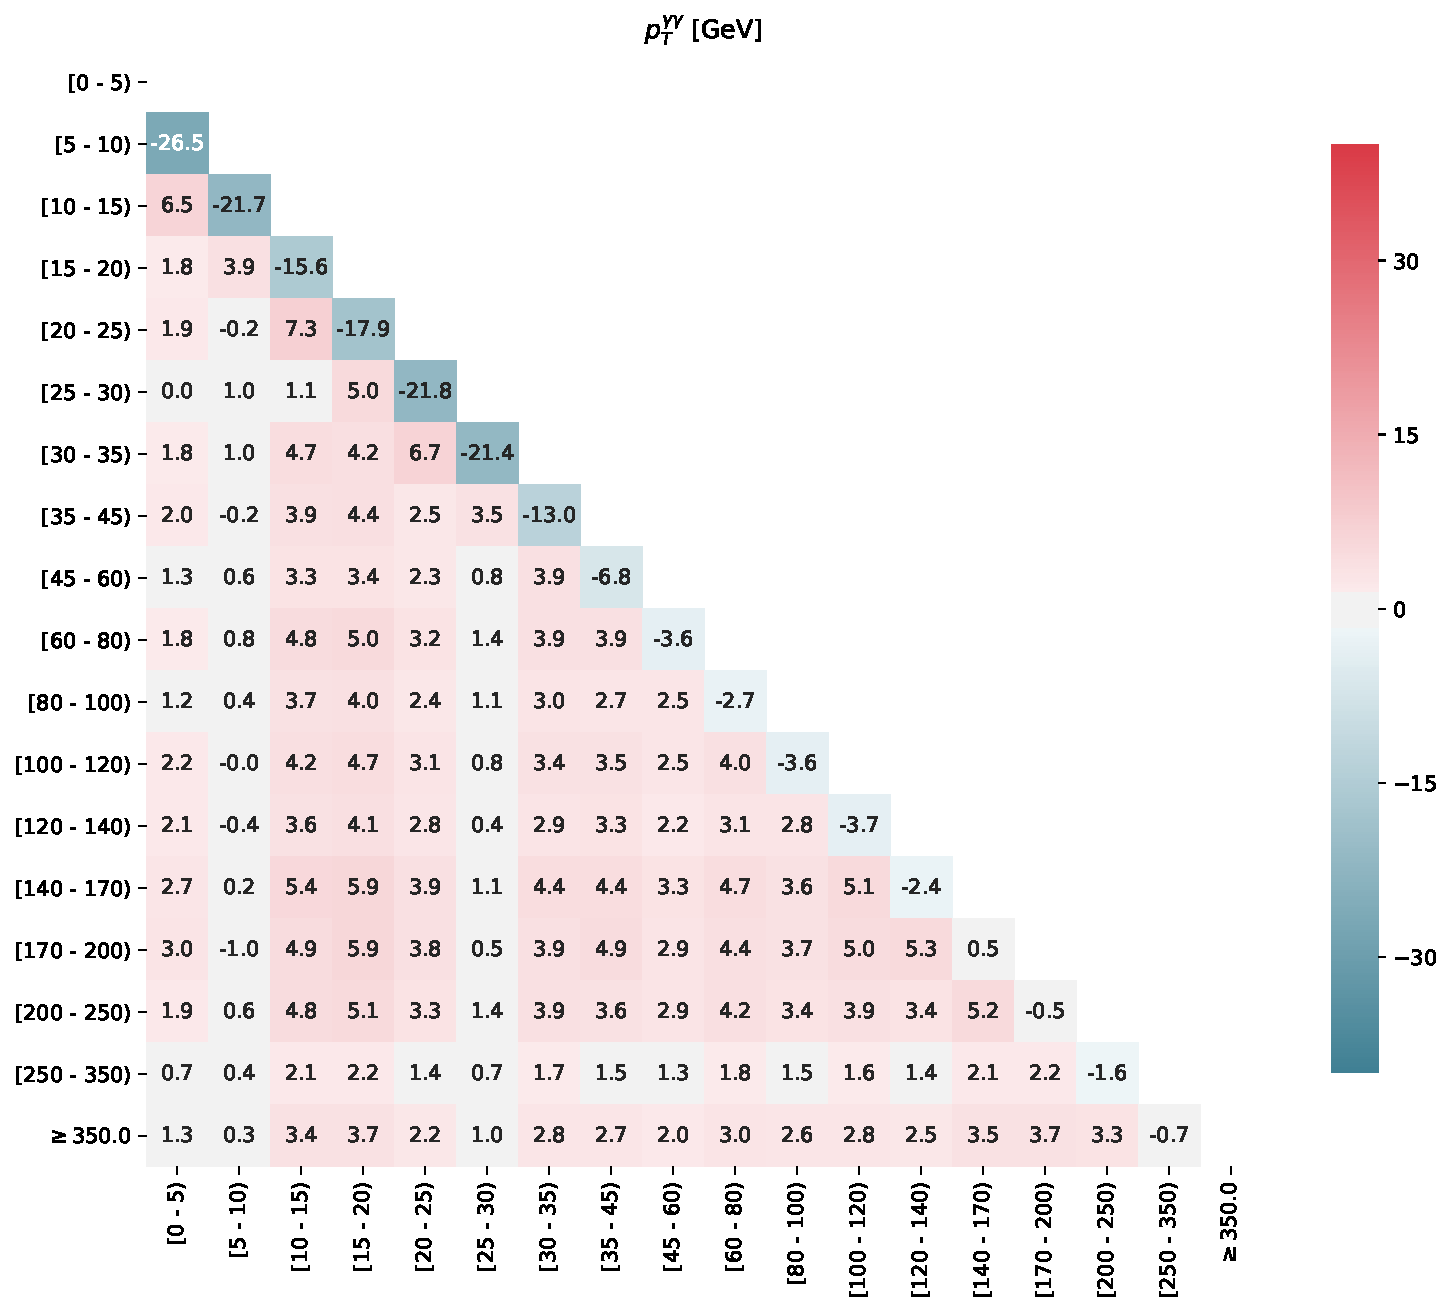
\includegraphics[scale=0.4]{plot-correlation/matrix/pT_yy/correlation_pT_yy_combDatabinned.pdf}
\caption{Correlation matrix in \% of the fitted cross sections' categories for $p_T^{\gamma\gamma}$, using the matrix unfolding method.In this case the matrix is nof perfectly diagonal, showing small correlations in the diagonal neighbouring categories.}
\label{correlation_matrix_unfolding}
\end{figure}
\\Most of the systematics are not constrained by the fit, except for the ones relative to the photon energy scale, the photon energy resolution and the error on the Higgs mass.
\\Fit results for each bin of each quantity under investigation and systematic pulls like the example shown in Figure \ref{pull_example} are shown in appendices.
\newpage
\phantom{i}
\vspace{3cm}
\begin{figure}[h]
\centering
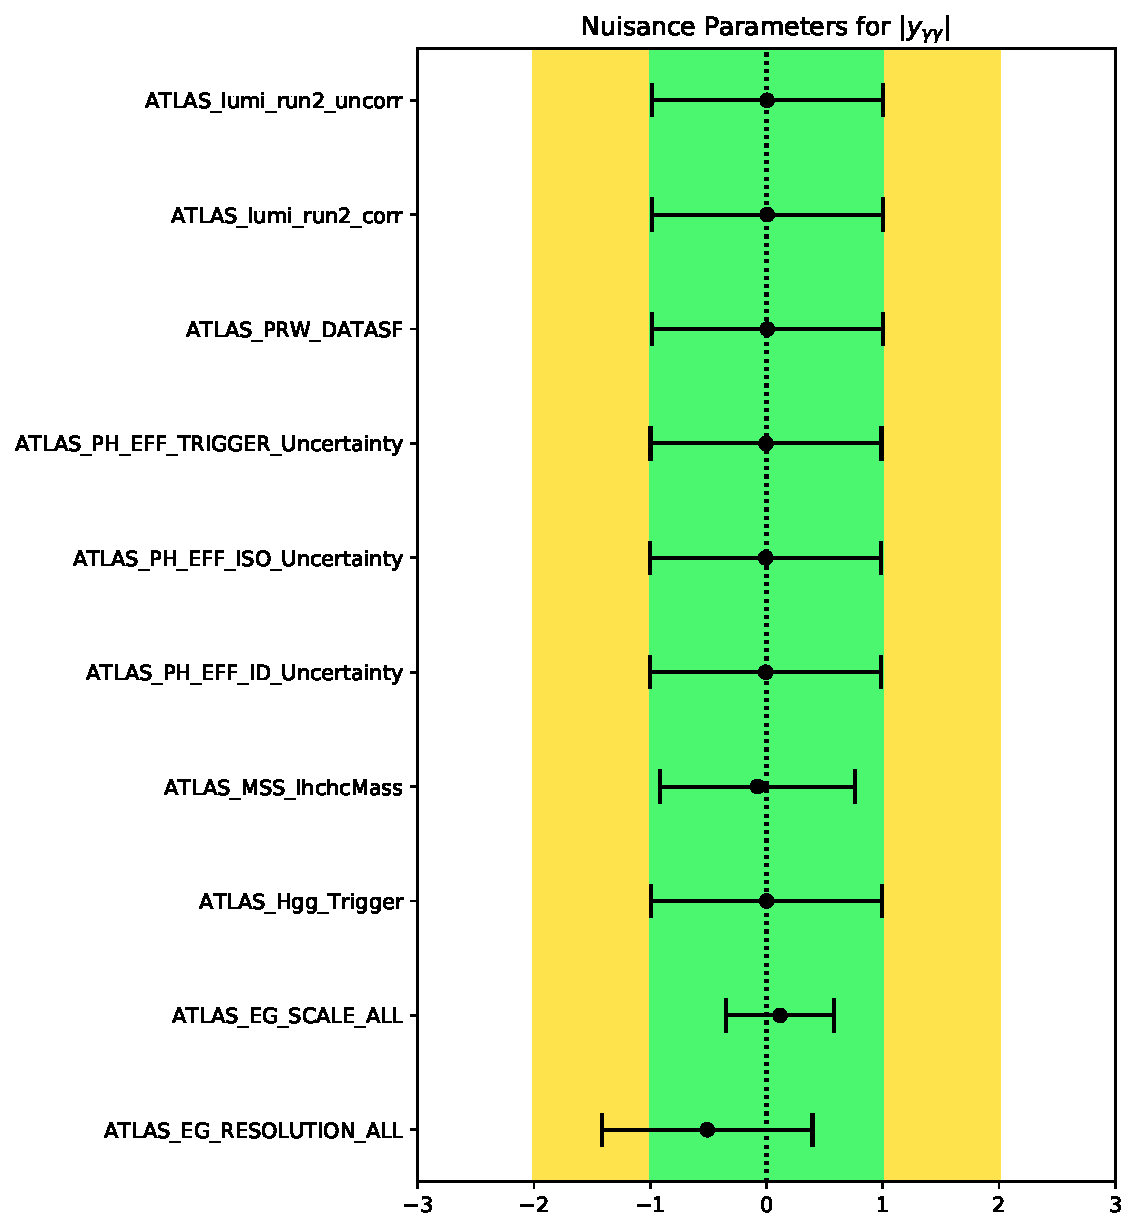
\includegraphics[width=\textwidth]{systematic_pulls_combDatabinned.pdf}
\caption{Systematic pulls of the real data fitting procedure for the $p_T^{\gamma\gamma}$ distribution.}
\label{pull_example}
\end{figure}
\newpage
\begin{figure}[H]
\centering
\subfloat{\includegraphics[scale=0.35]{plot-xsection/binbybin/pT_yy/xsection_pT_yy_AsimovSB.pdf}} \qquad
\subfloat{\includegraphics[scale=0.35]{plot-xsection/binbybin/yAbs_yy/xsection_yAbs_yy_AsimovSB.pdf}} \\
\subfloat{\includegraphics[scale=0.35]{plot-xsection/binbybin/Dphi_j_j_30_signed/xsection_Dphi_j_j_30_signed_AsimovSB.pdf}} \qquad
\subfloat{\includegraphics[scale=0.35]{plot-xsection/binbybin/N_j_30/xsection_N_j_30_AsimovSB.pdf}} \\
\subfloat{\includegraphics[scale=0.35]{plot-xsection/binbybin/pT_j1_30/xsection_pT_j1_30_AsimovSB.pdf}} \qquad
\subfloat{\includegraphics[scale=0.35]{plot-xsection/binbybin/m_jj_30/xsection_m_jj_30_AsimovSB.pdf}}
\caption{Plots for measured expected cross sections using the Asimov dataset and compared to the SM predictions for the different variables using bin-by-bin unfolding method.}
\end{figure}
\begin{figure}[H]
\centering
\subfloat{\includegraphics[scale=0.35]{plot-xsection/matrix/pT_yy/xsection_pT_yy_AsimovSB.pdf}} \quad
\subfloat{\includegraphics[scale=0.24]{plot-correlation/matrix/pT_yy/correlation_pT_yy_AsimovSB.pdf}} \\
\subfloat{\includegraphics[scale=0.35]{plot-xsection/matrix/yAbs_yy/xsection_yAbs_yy_AsimovSB.pdf}} \quad
\subfloat{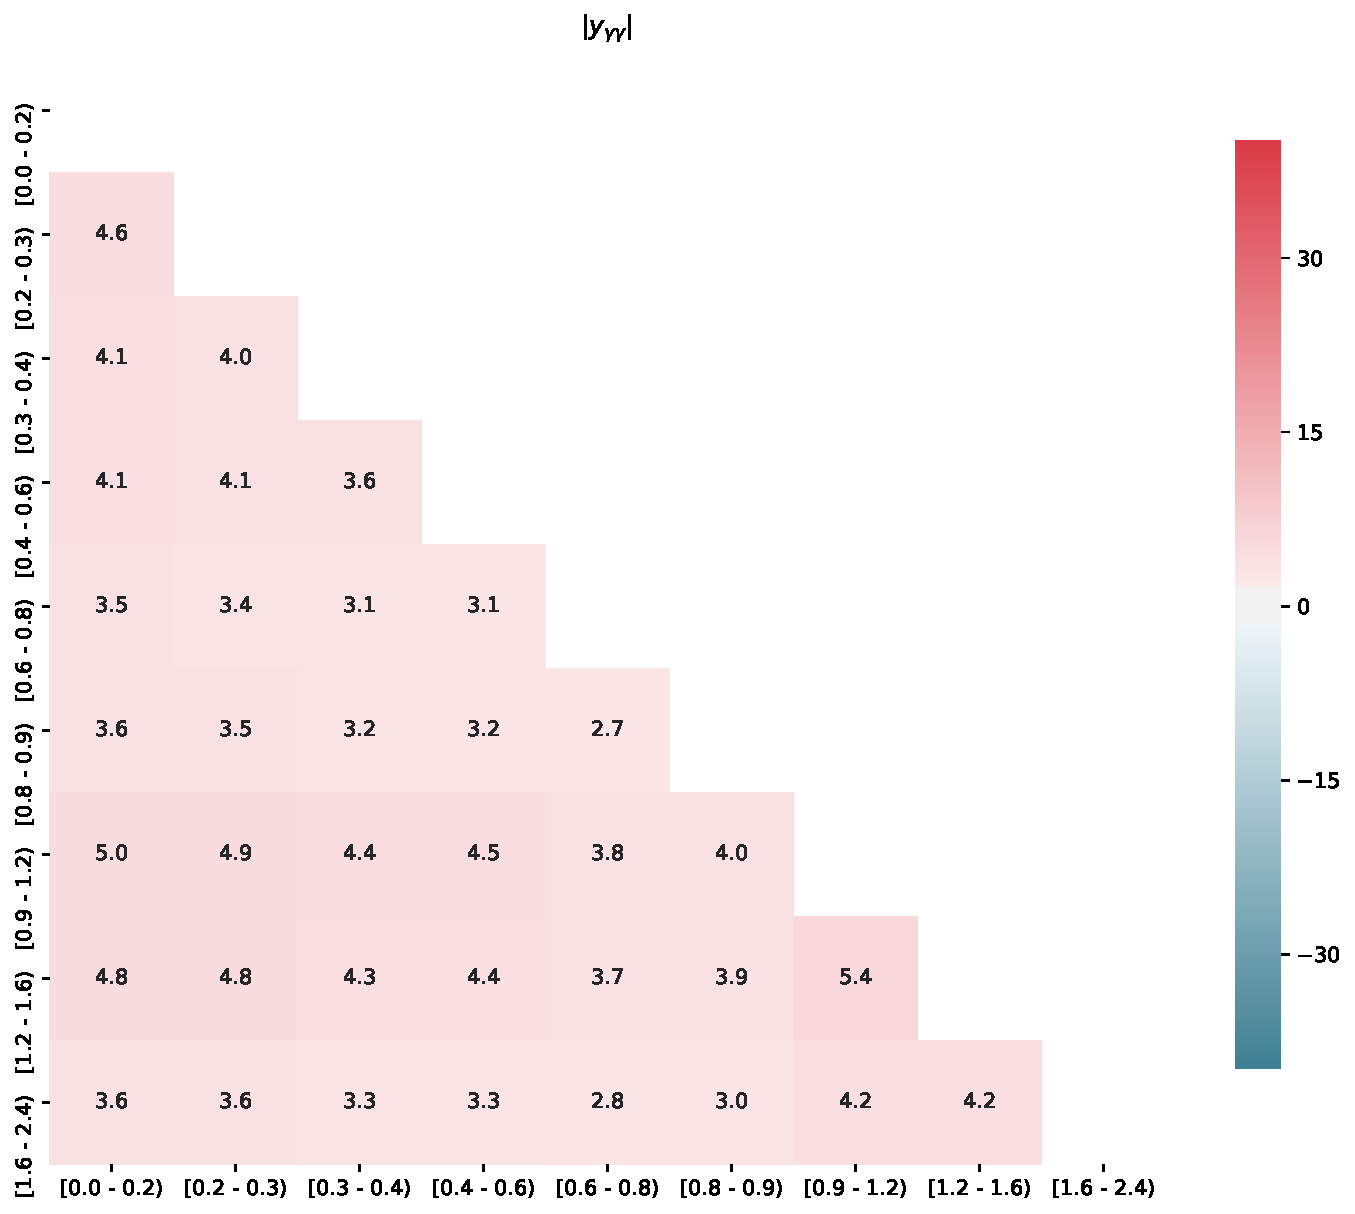
\includegraphics[scale=0.24]{plot-correlation/matrix/yAbs_yy/correlation_yAbs_yy_AsimovSB.pdf}} \\
\subfloat{\includegraphics[scale=0.35]{plot-xsection/matrix/Dphi_j_j_30_signed/xsection_Dphi_j_j_30_signed_AsimovSB.pdf}} \quad
\subfloat{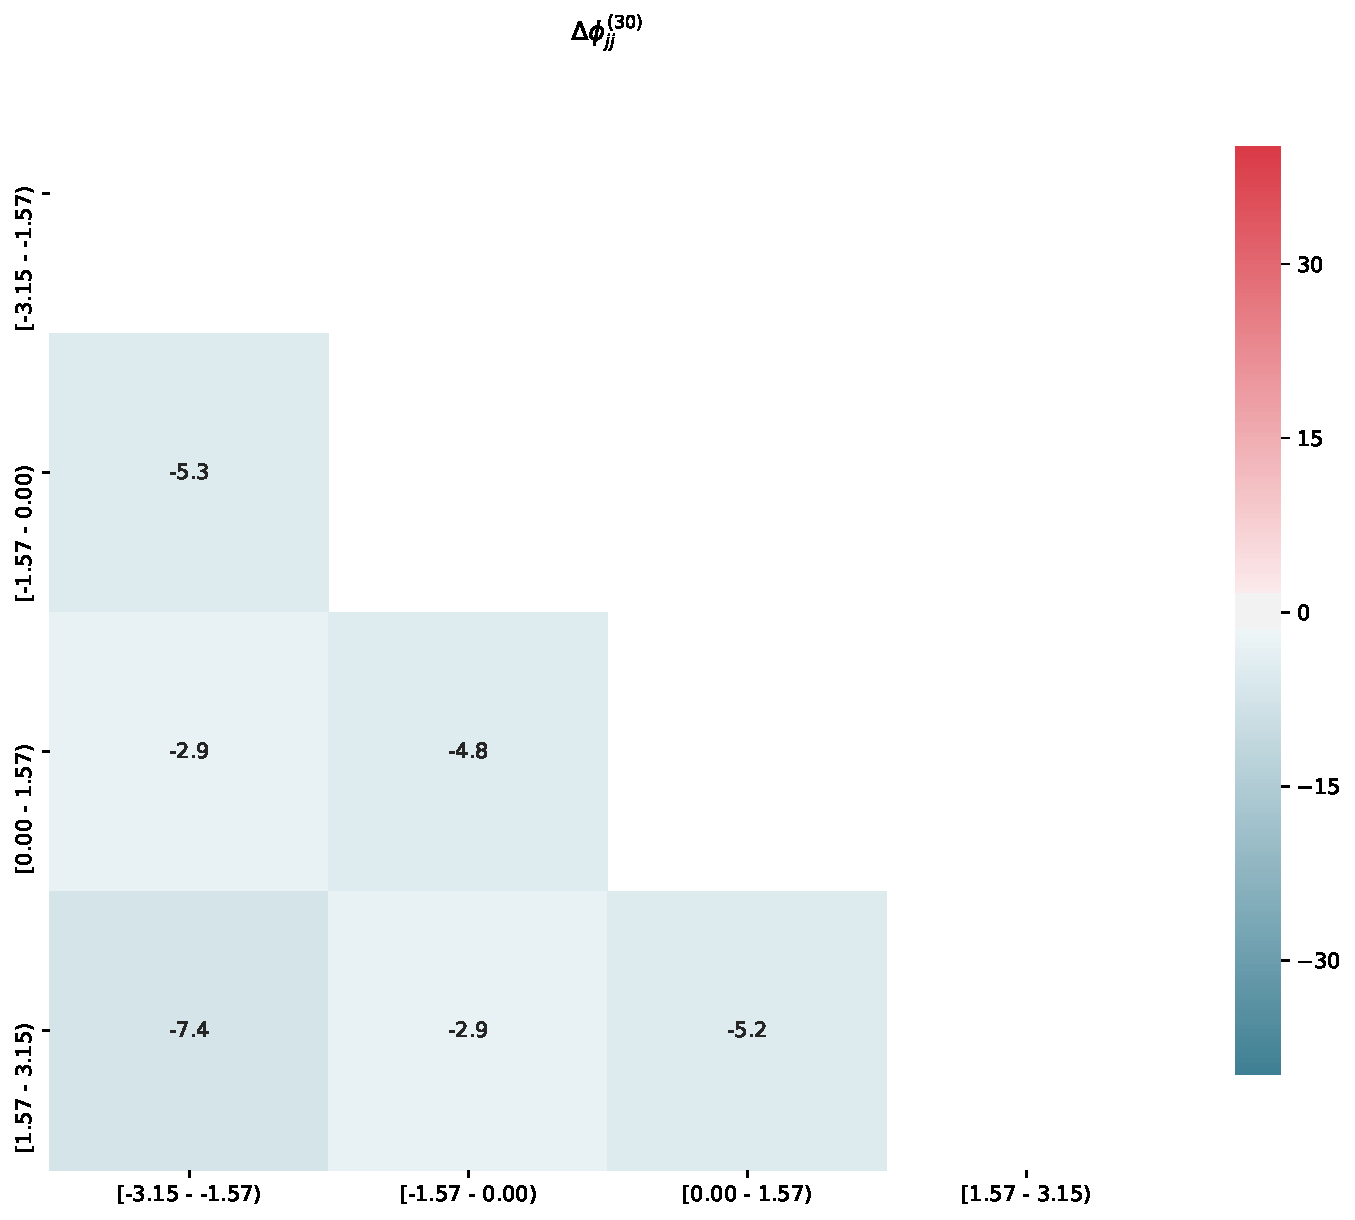
\includegraphics[scale=0.24]{plot-correlation/matrix/Dphi_j_j_30_signed/correlation_Dphi_j_j_30_signed_AsimovSB.pdf}}
\caption{Plots for measured expected cross sections using the Asimov dataset and compared to the SM predictions for the different variables using matrix unfolding method. In addition, the correlation matrix for each distribution are shown aside.}
\end{figure}
\begin{figure}[H]
\centering
\subfloat{\includegraphics[scale=0.35]{plot-xsection/matrix/N_j_30/xsection_N_j_30_AsimovSB.pdf}} \quad
\subfloat{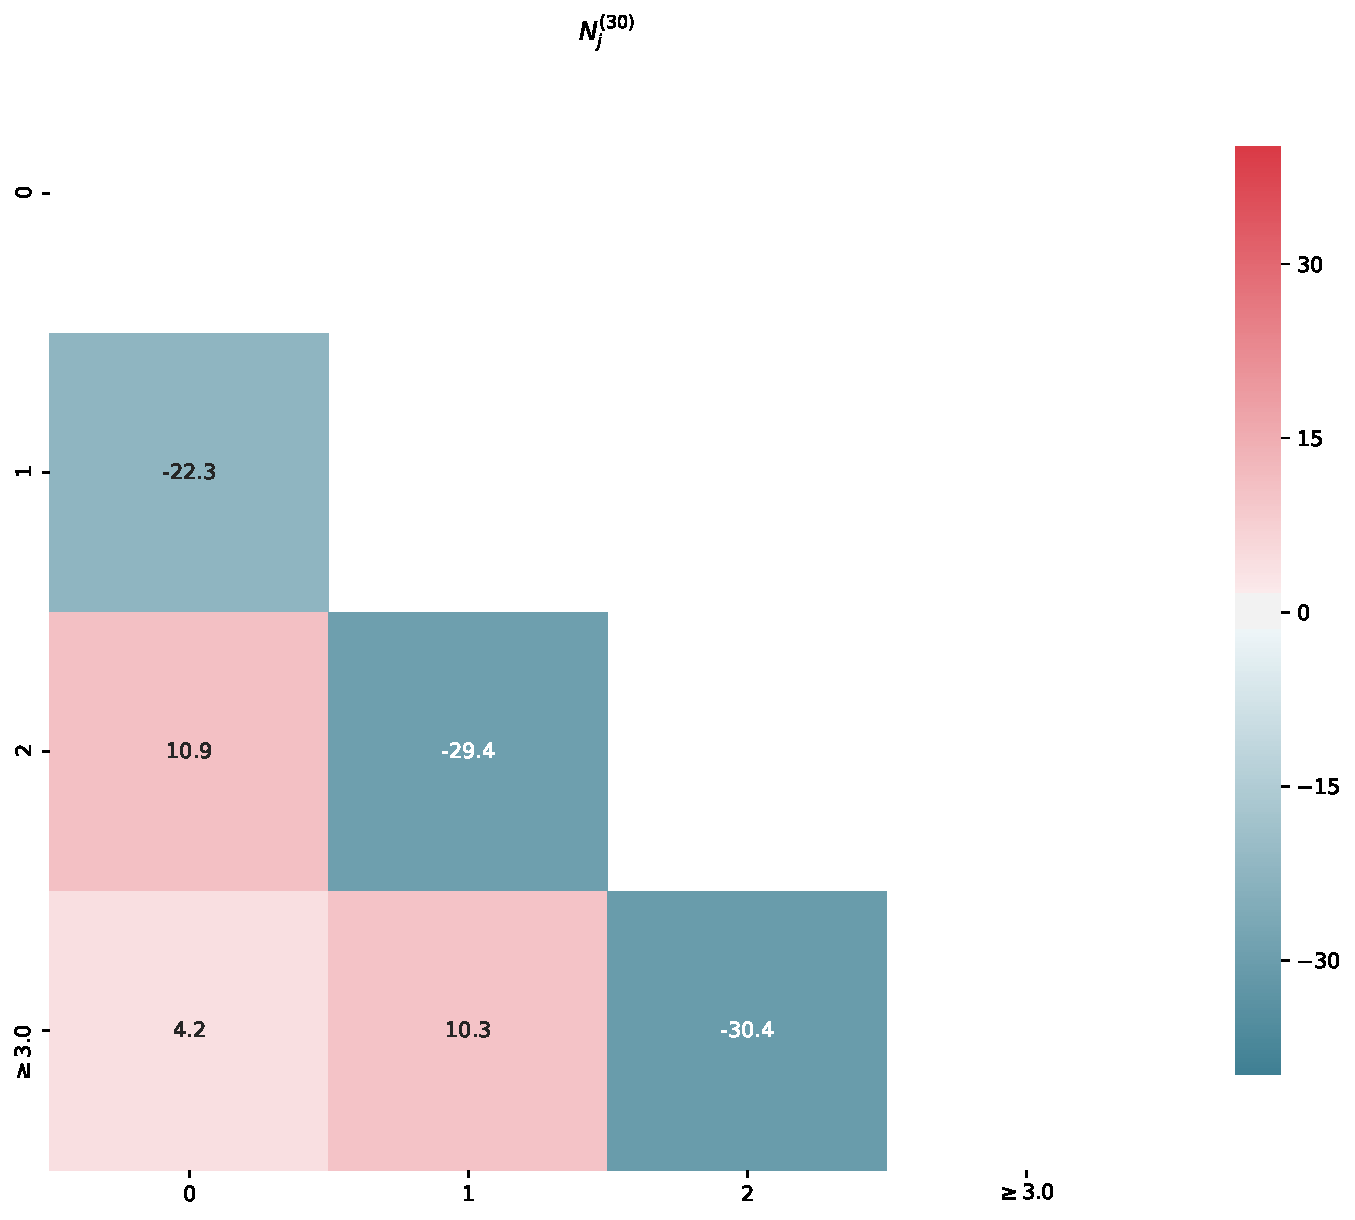
\includegraphics[scale=0.24]{plot-correlation/matrix/N_j_30/correlation_N_j_30_AsimovSB.pdf}} \\
\subfloat{\includegraphics[scale=0.35]{plot-xsection/matrix/pT_j1_30/xsection_pT_j1_30_AsimovSB.pdf}} \quad
\subfloat{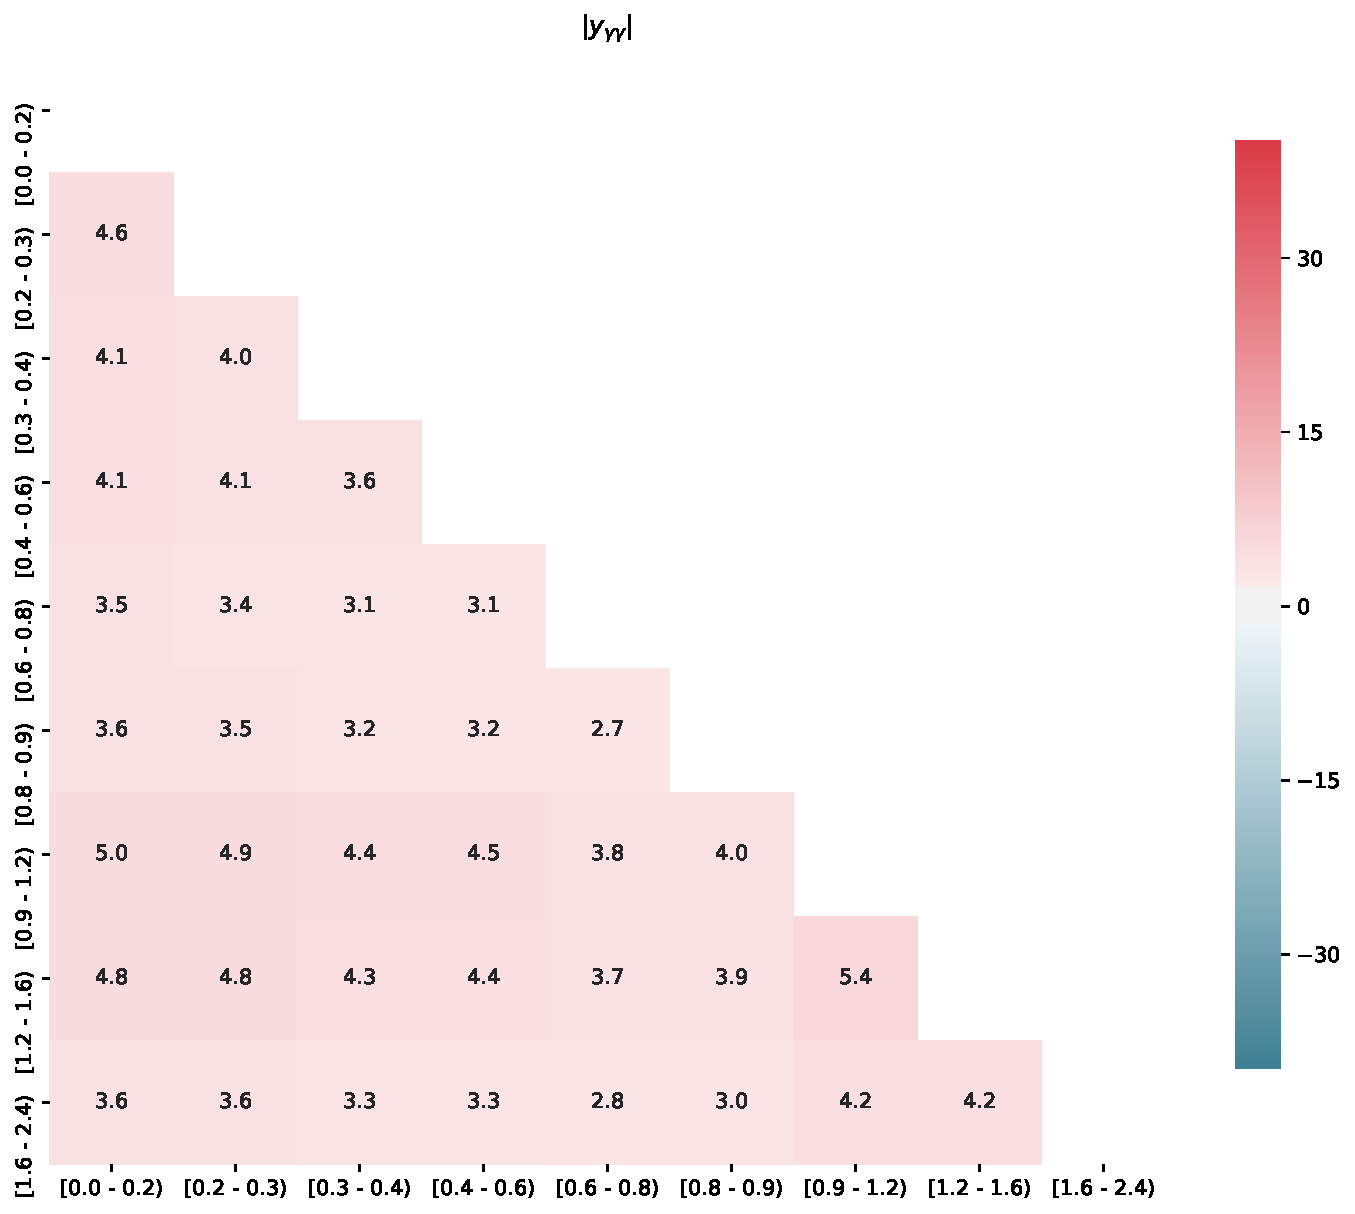
\includegraphics[scale=0.24]{plot-correlation/matrix/yAbs_yy/correlation_yAbs_yy_AsimovSB.pdf}} \\
\subfloat{\includegraphics[scale=0.35]{plot-xsection/matrix/m_jj_30/xsection_m_jj_30_AsimovSB.pdf}} \quad
\subfloat{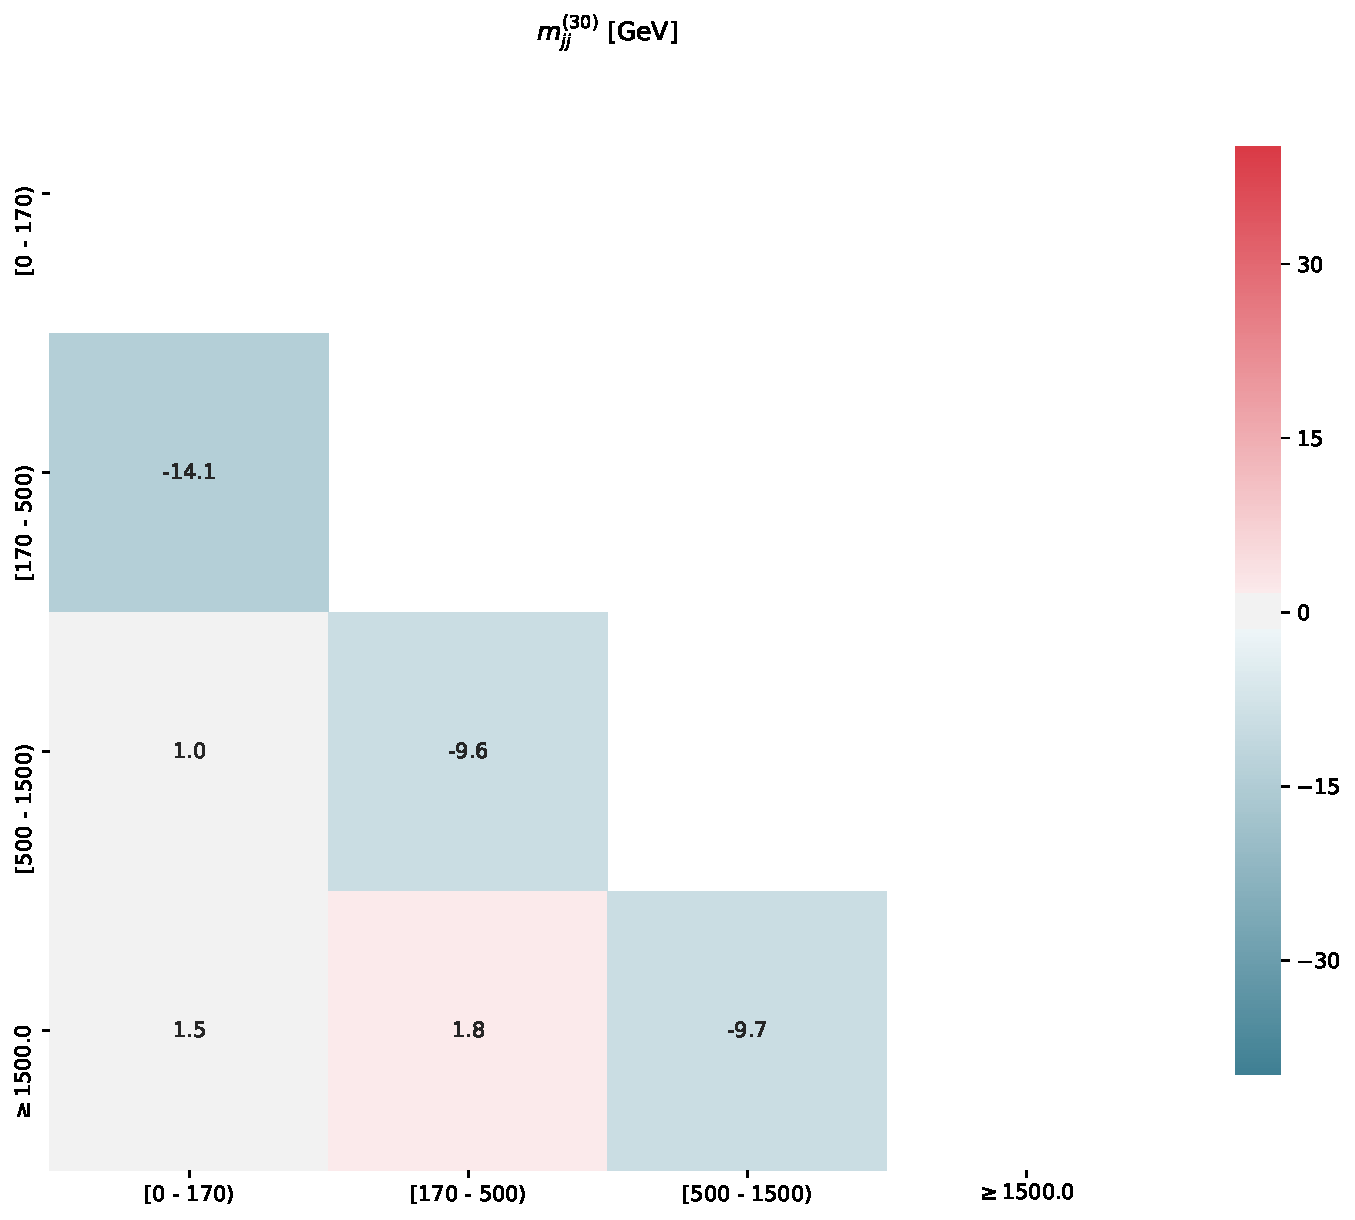
\includegraphics[scale=0.24]{plot-correlation/matrix/m_jj_30/correlation_m_jj_30_AsimovSB.pdf}}
\caption{Plots for measured expected cross sections using the Asimov dataset and compared to the SM predictions for the different variables using matrix unfolding method. In addition, the correlation matrix for each distribution are shown aside.}
\end{figure}


\section{Observed results}
The fitted $m_{\gamma\gamma}$ distribution is shown for an example category in Figure \ref{fit_example}. The observed results for the fiducial differential cross sections multiplied for the Branching Ratio for the $H \rightarrow \gamma\gamma$ decay channel are obtained fitting the real data. The results are compared to the Standard Model predictions for the separate differential variables distributions. Both bin-by-bin unfolding method and matrix unfolding method have been used in the analysis.
\begin{figure}[t]
\centering
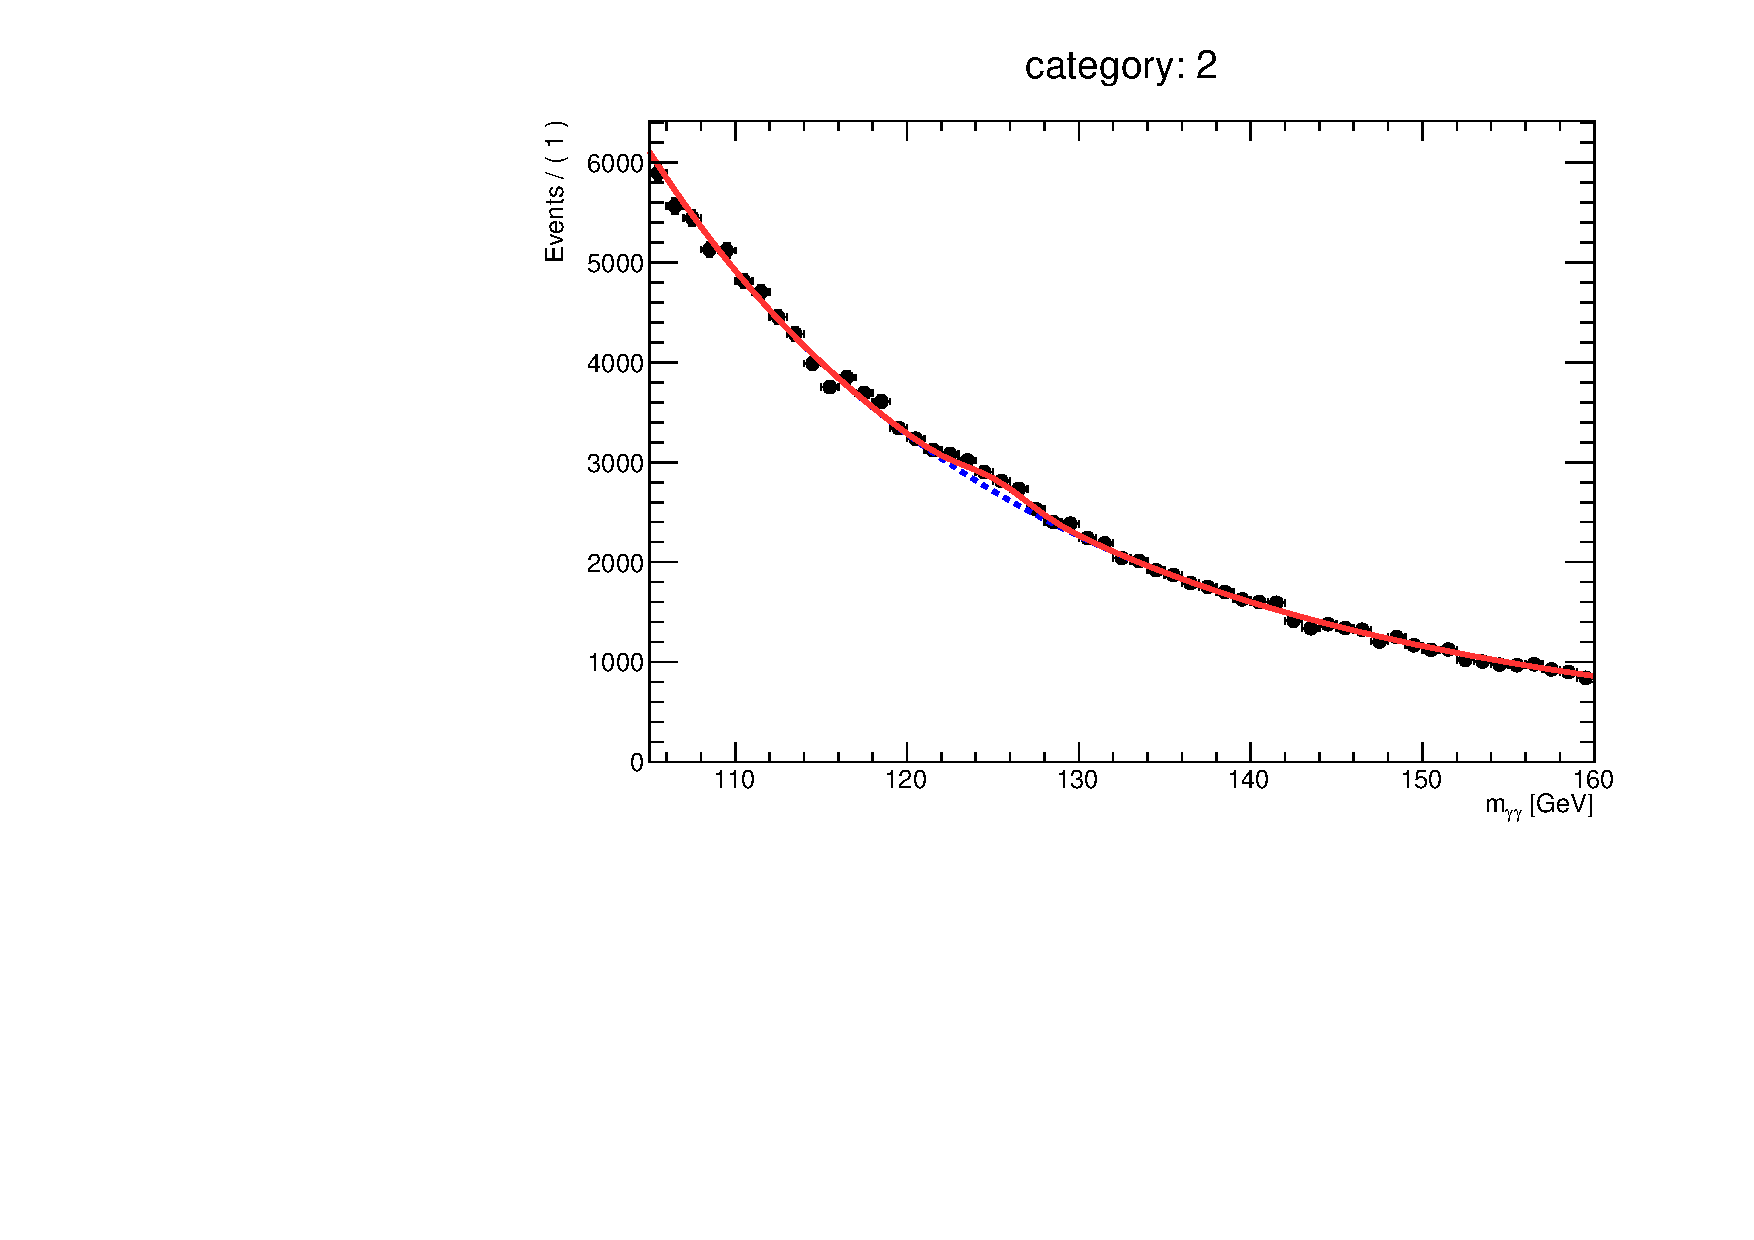
\includegraphics[scale=0.4]{fit_plots_final/pT_yy/XSectionWS_pT_yy__category_2.pdf}
\caption{Example of $m_{\gamma\gamma}$ distribution fit for $p_T^{\gamma\gamma}$ in range $5\text{GeV} < p_T^{\gamma\gamma} < 10 \text{GeV}$.}
\label{fit_example}
\end{figure}
\\Differential cross-sections results for analysis performed using both unfolding methods are shown in Figure \ref{combDatabinned_bin-by-bin} and in Figure \ref{combDatabinned_matrix}. The good agreement between the measured observed cross sections and the SM predictions is observed.
\begin{figure}[htb]
\centering
\subfloat{\includegraphics[scale=0.33]{plot-xsection/binbybin/pT_yy/xsection_pT_yy_combDatabinned.pdf}} \qquad
\subfloat{\includegraphics[scale=0.33]{plot-xsection/binbybin/yAbs_yy/xsection_yAbs_yy_combDatabinned.pdf}} \\
\subfloat{\includegraphics[scale=0.33]{plot-xsection/binbybin/Dphi_j_j_30_signed/xsection_Dphi_j_j_30_signed_combDatabinned.pdf}} \qquad
\subfloat{\includegraphics[scale=0.33]{plot-xsection/binbybin/N_j_30/xsection_N_j_30_combDatabinned.pdf}}
\end{figure}
\begin{figure}[htb]
\centering
\subfloat{\includegraphics[scale=0.33]{plot-xsection/binbybin/pT_j1_30/xsection_pT_j1_30_combDatabinned.pdf}} \qquad
\subfloat{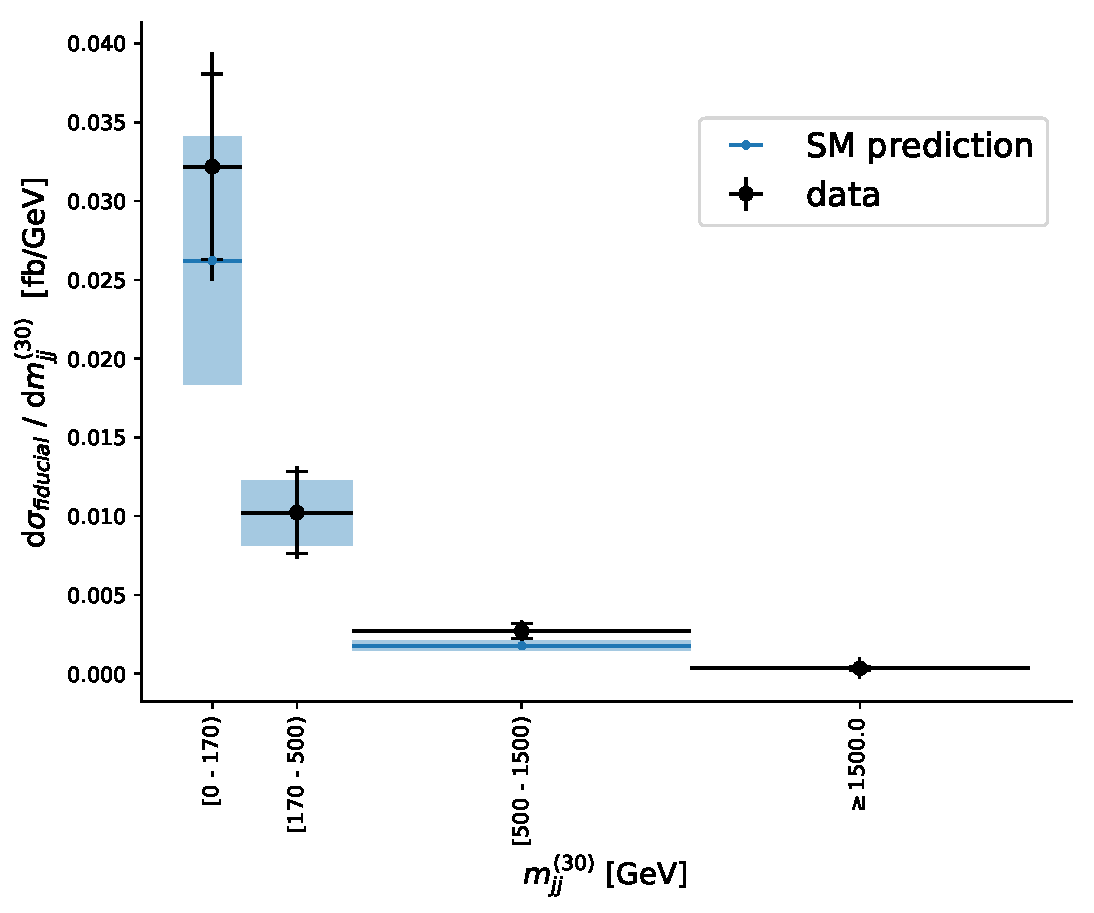
\includegraphics[scale=0.33]{plot-xsection/binbybin/m_jj_30/xsection_m_jj_30_combDatabinned.pdf}}
\caption{Plots for measured observed cross sections using the dataset and compared to the SM predictions for the different variables using bin-by-bin unfolding method.}
\label{combDatabinned_bin-by-bin}
\end{figure}
\begin{figure}[H]
\centering
\subfloat{\includegraphics[scale=0.33]{plot-xsection/matrix/pT_yy/xsection_pT_yy_combDatabinned.pdf}} \qquad
\subfloat{\includegraphics[scale=0.33]{plot-xsection/matrix/yAbs_yy/xsection_yAbs_yy_combDatabinned.pdf}} \\
\subfloat{\includegraphics[scale=0.33]{plot-xsection/matrix/Dphi_j_j_30_signed/xsection_Dphi_j_j_30_signed_combDatabinned.pdf}} \qquad 
\subfloat{\includegraphics[scale=0.33]{plot-xsection/matrix/N_j_30/xsection_N_j_30_combDatabinned.pdf}}
\end{figure}
\begin{figure}[t]
\centering
\subfloat{\includegraphics[scale=0.33]{plot-xsection/matrix/pT_j1_30/xsection_pT_j1_30_combDatabinned.pdf}} \qquad
\subfloat{\includegraphics[scale=0.33]{plot-xsection/matrix/m_jj_30/xsection_m_jj_30_combDatabinned.pdf}} \\
\caption{Plots for measured observed cross sections using the dataset and compared to the SM predictions for the different variables using matrix unfolding method.}
\label{combDatabinned_matrix}
\end{figure}
\newpage

\section{Extrapolation for High-Luminosity LHC}
The Large Hadron Collider, successfully commissioned in 2010 and so far the world's largest and highest-energy particle collider, has enabled physicists to investigate and test with high precision all the key questions of the sub-atomic world and and perform several searches of new physics beyond the Standard Model. A possible development ugprade is to increase the luminosity and thus the beam collision rate, in order to extend its discovery potential. This new scenario and machine configuration is called \emph{High- Luminosity LHC} (HL-LHC) and aims to push the luminosity by a factor of five beyond its design value, expecting to deliver the integrated luminosity design goal up to $3000$ fb $^{-1}$.
\\
The very high instananeous luminosity will lead to about 200 proton-proton collisions per bunch crossing superimposed to each selected event\cite{Apollinari_2017cqg, sekmen2019standard}.
\begin{figure}[b!]
\centering
\includegraphics[scale=0.35]{pT_yy_HI_LUMI_LHC_extrapolation.pdf}
\caption{Integrated luminosity extrapolation for High-Luminosity LHC configuration for $p_T^{\gamma\gamma}$ distribution, using the bin-by-bin unfolding.}
\label{extrapolation}
\end{figure}
\\In this work an extrapolation on how increasing luminosity will reflects on the uncertainties sources is produced. In Figure \ref{extrapolation} the $p_T^{\gamma\gamma}$ distribution has been used in the extrapolation, investigating the integrated luminosity range $70 \text{fb}^{-1} < L < 5000 \text{fb}^{-1}$.
\\\\
In some bins the behaviour is dominated by the reduction of the statistical error, thanks to the higher luminosity, while others start to be domaniated by the systematic errors, in particular by the spurious signal sistematic.
\\\\
From this extrapolation you can notice how the High-Luminosity LHC configuration will bring lots of improvements, at the cost to push the statistical machinery at its limit, in order to process a huge amount of data. 